\documentclass[a4paper,12pt]{article}
\usepackage[top=12ex, bottom=12ex, left=9ex, right=9ex,showframe=false]{geometry}
\linespread{1.8}
\usepackage[ampersand]{easylist}
\usepackage{fancyhdr}
\pagestyle{fancy}
\lhead{ \fancyplain{}{Yuhao Yang} }
\rhead{ \fancyplain{}{\leftmark} }
\cfoot{ \fancyplain{}{\thepage} }
\usepackage[unicode]{hyperref}
\usepackage{amsmath}
\usepackage{amsfonts}
\usepackage{latexsym}
\usepackage{pifont}
\usepackage{fourier}
\usepackage[dvipsnames,svgnames]{xcolor}
\usepackage{extarrows}
\usepackage{graphicx}
\usepackage{tikz}
\usepackage{pgfplots}
\usetikzlibrary{arrows,positioning,calc,fadings,shapes,decorations.markings}
\usepackage{array}
\usepackage{anyfontsize}
\usepackage{indentfirst}
\usepackage{ulem}
\usepackage{paralist}
\usepackage{enumitem}
\usepackage{framed}
\usepackage{tcolorbox}
\usepackage{wrapfig}
\usepackage{xfrac}

% % % % % % % % % %

% font type
\renewcommand*\rmdefault{ppl}
%\newcommand{\dd}{\mathrm{d}}
%\newcommand{\ee}{\mathrm{e}}

% % % % % % % % % %

\renewcommand\thefootnote{\textcolor{blue}{[\arabic{footnote}]}}
\hypersetup{
    colorlinks, linkcolor={purple}, citecolor={blue}, urlcolor={blue},
    pdftitle={Cambridge International A-Level Physics Course Handout},
    pdfauthor={Yuhao Yang},
    pdfsubject={A-Level Physics} }

% tikz arrows
\tikzset{>=stealth', pil/.style={ ->, thick, shorten <=2pt, shorten >=2pt,} }

% tikz decription node style
\tikzset{note/.style={rectangle, rounded corners, minimum size=6mm, draw=black, fill=white, font=\itshape, align=center,execute at begin node=\setlength{\baselineskip}{1.2em}}}
\tikzset{graphlabel/.style={postaction={decorate,transform shape, decoration={markings, mark=at position .5 with \node #1;}}}}

% % % % % % % % % % %

% example environment
\newcounter{example}[section]
\renewcommand{\theexample}{\arabic{section}.\arabic{example}}

\newcommand{\example}[1]{\refstepcounter{example}
	\vspace*{0.5\baselineskip}\noindent{\textsf{\textbf{Example \theexample }} \hspace*{1pt} #1 %
	}}
\newcommand{\eoe}{\hfill $\square$}
\newcommand{\teoe}{\tag*{$\square$}}

\newcommand{\keypoint}[1]{\textbf{\textcolor{red}{#1}}}
\newcommand{\cmt}{\noindent\hspace{-0.4em}\ding{43} \hspace{0.4em}}

% indentation and line spacing in itemize environment
\setitemize{noitemsep,topsep=0pt,parsep=0pt,partopsep=0pt}
\numberwithin{equation}{section}
\numberwithin{figure}{section}
\everymath{\displaystyle}

% indentation of paragraphs and table of contents
\setlength{\parindent}{1.2em}

% columns with customised width in tabulars
\newcolumntype{C}[1]{>{\centering\arraybackslash}p{#1}}
\newcolumntype{D}[1]{ >{\centering\arraybackslash} m{1cm} }

\title{Further Mechanics}
\author{Yuhao Yang}

\newcommand{\dd}{\mathrm{d}}
\newcommand{\opdt}{\frac{\mathrm{d}}{\mathrm{d}t}}
\newcommand{\ddt}[1]{\frac{\mathrm{d}#1}{\mathrm{d}t}}
\newcommand{\dddt}[1]{\frac{\mathrm{d}^2#1}{\mathrm{d}t^2}}
\newcommand{\RA}{\quad \Rightarrow \quad}
\newcommand{\mps}{\text{ (m s$^{-1}$)}}
\newcommand{\mpss}{\text{ (m s$^{-2}$)}}
\newcommand{\tmax}{\text{max}}
\newcommand{\tmin}{\text{min}}
\newcommand{\rad}{\text{ rad}}
\newcommand{\radps}{\text{ (rad s$^{-1}$)}}
\newcommand{\eqskip}{\hspace{2.0em}}
\newcommand{\yskip}{\vspace{0.6em}}

\begin{document}
	

\vspace*{5pt}

\begin{center}
	{
		\Huge Further Mechanics
	
	}
	
	{
		\Large Yuhao Yang
		
		Easyday Education
	
	}

	
\end{center}

\vspace*{5pt}

\setcounter{page}{1}
\pagenumbering{roman} 
\tableofcontents
%\listoffigures

\newpage

\section*{A Few Words about the Notes}


This is a set of very concise lecture notes written for A-level further mechanics. I intend to introduce the physical concepts and principles required by the syllabus using a more mathematical approach, so that the reader may develop an appreciation of the interplay between mathematics and physics. A handful of worked examples are included to give the reader some rough idea about how exam-style questions look like and how the principles developed in the note can be applied to solve them. The complexity to type mathematical equations and draw diagrams on a computer gave me a good excuse to skip several interesting example questions.

Presumably the target audience of the notes are students studying the relevant A-Level course. If you are a student hoping for good grades in your exams, I suggest you have your hand on a lot of problems. The notes are supposed to be used as a reference only, but it is eventually by practising one can have a better understanding of the subject.

I have to admit that these notes are far from complete. I hope you enjoy reading the notes. But if you spot any mistake (as I guarantee there will be a lot), please let me know.

{

\flushright

Yuhao Yang

\url{colin.young@live.com}

\today

}


\newpage
\setcounter{page}{1}
\pagenumbering{arabic}

\section{Momentum \& Impulse}


\subsection{momentum \& impulse}

we define momentum as product of mass and velocity: $\boxed{p = mv}$

consider rate of change in momentum: $\frac{\dd p}{\dd t} = \opdt (mv) = m \ddt{v} = F $

this gives Newton's second law: resultant force equals rate of change in momentum

separate variables and integrate: $\int \dd p = \int F \dd t \RA \Delta p = \int F \dd t$

we define impulse of a force as: $\boxed{J = \int F \dd t}$ 

if the force acting is constant, then impulse $J=F\Delta t$

we have the impulse-momentum relation: $\boxed{J = \Delta p}$

i.e., impulse causes change in momentum

\vspace*{\baselineskip}

note that both momentum and impulse are vectors, i.e., they have directions

momentum of a moving object is in same direction as its velocity

impulse of a force is in same direction as the force

\example{An object of mass 2 kg is initially at rest, if it is acted by a force of 6 N for of 0.5 s, at what speed is the object moving?}

{

\centering

$\Delta p = J \RA mv - 0 = F\Delta t \RA v=\frac{F\Delta t}{m} = \frac{6\times0.5}{2}=1.5 \mps $

}

\example{A bullet of mass 10 g enters a wooden block at 250 m/s. After a time of 0.005 s, the bullet leaves the block at 50 m/s. What is the average resistive force acting?}

{
	
	\centering
	
	$\Delta p = J \RA mv - mu = F\Delta t \RA F = \frac{m(v-u)}{\Delta t} = \frac{0.010\times(50-250)}{0.005} = -400$ (N)
	
}

magnitude of resistive force is 400 N, minus sign means it is opposite to bullet's motion

\subsection{conservation of momentum}

for point mass in absence of net external force, $\Delta p = 0$, i.e., momentum is constant


for a system of point objects $m_i$, each experiences a force $F_i$

$F_i$ can come from external source or another object $j$ within system: $F_i = F_{i,\text{ext}} + \sum_j F_{i,j}$

summing over all objects: $\sum_i F_i = \sum_i F_{i,\text{ext}} + \sum_{i,j} F_{i,j}$

for each pair $i$ and $j$, recall action-reaction principle: $F_{i,j} = -F_{j,i}$

so $\sum_{i,j} F_{i,j} = 0$, then $\sum_i F_i = \sum_i F_{i,\text{ext}}$

note that $\sum_i F_i \Delta t = \sum_i J_i = \sum_i \Delta p_i  \RA \boxed{\left(\sum_i F_{i,\text{ext}} \right)\Delta t = \sum_i \Delta p_i}$

\vspace*{\baselineskip}

change in total momentum of system depends on net external impulse acting

in particular, if there is no net external impulse, total momentum remains constant

this is called the conservation of momentum

\subsection{collision problems}

if two objects collide, $\Delta t \approx 0$, external force produces negligible impulse

so momentum is always conserved for a collision process

\begin{figure}[htp]
\noindent\begin{minipage}{0.5\textwidth}
	\begin{center}
		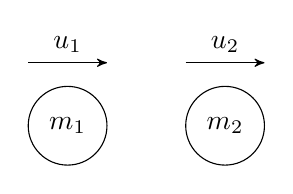
\begin{tikzpicture}
		\draw (-1,0) circle (0.5) node{$m_1$};
		\draw (1,0) circle (0.5) node{$m_2$};
		\draw[->] (-1.5,.8) -- (-0.5,.8) node[midway,above]{$u_1$};
		\draw[->] (0.5,.8) -- (1.5,.8) node[midway,above]{$u_2$};
		\end{tikzpicture}
		
		initial state before collision
	\end{center}
\end{minipage}
\begin{minipage}{0.5\textwidth}
	\begin{center}
		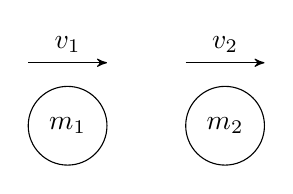
\begin{tikzpicture}
		\draw (-1,0) circle (0.5) node{$m_1$};
		\draw (1,0) circle (0.5) node{$m_2$};
		\draw[->] (-1.5,.8) -- (-0.5,.8) node[midway,above]{$v_1$};
		\draw[->] (0.5,.8) -- (1.5,.8) node[midway,above]{$v_2$};
		\end{tikzpicture}
		
		final state after collision
	\end{center}
\end{minipage}
\end{figure}

before and after collision, one has: $\boxed{m_1u_1 + m_2u_2 = m_1v_1 + m_2v_2}$

due to the vector nature of momentum, minus sign is needed if direction of motion reverses

\subsubsection{elastic \& inelastic collisions}

for inelastic collision, kinetic energy is lost to plastic deformation

for elastic collisions, no kinetic energy is lost: $\boxed{\frac{1}{2}m_1 u_1^2 + \frac{1}{2}m_2 u_2^2 = \frac{1}{2}m_1 v_1^2 + \frac{1}{2}m_2 v_2^2}$

together with momentum conservation, this reduces to $\boxed{u_1 - u_2 = v_2 - v_1}$

for elastic collision, relative speed of approach equals relative speed of separation 

for inelastic process, relative speed of separation is less than that of approach

\subsubsection{coefficient of restitution}

define coefficient of restitution as ratio of relative speeds before and after collision:
\begin{center}
$\boxed{e = \frac{v_2 - v_1}{u_1 - u_2}}$ or $\boxed{v_2 - v_1 = e(u_1 - u_2)}$
\end{center}

for elastic collision, $e = 1$; for inelastic collision, $0 < e < 1$

\vspace*{\baselineskip}

if an object collides at right angle with a fixed barrier with initial speed $u$

since barrier does not move, so $v-0 = e(0-u)$, then $v=-eu$

so object moves at speed $v=eu$ after collision, but with direction reversed



\example{Two small spheres $A$ and $B$ have masses $3m$ and $m$. They are projected towards each other with speeds $2u$ and $u$ relatively, the collision is perfectly elastic. What are their final speeds?}

momentum conservation: $3m\cdot 2u - m \cdot u = 3m v_A + m v_B$

relation for relative speeds: $v_B - v_A = 2u + u$

take simultaneous equations: $\Bigg\{\begin{array}{l}
3v_A + v_B = 5u \\
v_B - v_A = 3u
\end{array} \RA 
\Bigg\{\begin{array}{l}
v_A = \frac{1}{2}u \\
v_B = \frac{7}{2}u
\end{array}$

positive $v_A$ and $v_B$ means both spheres move in same direction as $u_A$ after collision \eoe

\example{Sphere $A$ of mass $m$ and sphere $B$ of mass $km$ are initially at rest. Sphere $A$ is projected towards $B$ with speed $u$, the restitution of collision is $\frac{1}{3}$. After the collision, sphere $A$ reverses. What is the possible range for value of $k$?}

{
	
\centering

$\Bigg\{\begin{array}{l}
mu + 0 = m v_A + km v_B \\
v_B - v_A = \frac{1}{3}(u-0)
\end{array} \RA
\Bigg\{\begin{array}{l}
	v_A + k v_B = u\\
	v_B - v_A = \frac{1}{3}u
\end{array} \RA 
\Bigg\{\begin{array}{l}
v_A = \frac{(3-k)u}{3(1+k)} \\
v_B = \frac{4u}{3(1+k)}
\end{array}$

}

sphere $A$ reverses so $v_A<0$ after collision $\RA \frac{(3-k)u}{3(1+k)}<0 \RA 3-k <0 \RA k>3$ \eoe

\example{Two small spheres $A$ and $B$ of masses $3m$ and $m$ lie on a smooth horizontal surface at rest. Sphere $A$ is projected towards $B$ with speed $u$. After the collision $B$ goes on to collide directly with a fixed smooth vertical barrier, before colliding with $A$ again. The coefficient of restitution between the spheres is $\frac{2}{3}$ and the coefficient of restitution between $B$ and the barrier is $e$. After the second collision between $A$ and $B$, the speed of $B$ is nine times the speed of $A$. Find the possible values of $e$.}

first collision between $A$ and $B$:

{
	
	\centering
	
	$\Bigg\{\begin{array}{l}
	3mu + 0 = 3m v_A + m v_B \\
	v_B - v_A = \frac{2}{3}(u-0)
	\end{array} \RA
	\Bigg\{\begin{array}{l}
	3v_A + v_B = 3u\\
	v_B - v_A = \frac{2}{3}u
	\end{array} \RA 
	\Bigg\{\begin{array}{l}
	v_A = \frac{7}{12}u \\
	v_B = \frac{5}{4}u
	\end{array}$
	
}

collsion between $B$ and the barrier: $v_B' = -ev_B \RA v_B' = -\frac{5e}{4}u$

second collision between $A$ and $B$:

{
	
	\centering
	
	$\Bigg\{\begin{array}{l}
	3mv_A + mv_B' = 3m w_A + m w_B \\
	w_B - w_A = \frac{2}{3}(v_A-v_B')
	\end{array} \RA
	\Bigg\{\begin{array}{l}
	3w_A + w_B = 3\cdot\frac{7}{12}u - \frac{5e}{4}u = \frac{7-5e}{4}u\\
	w_B - w_A = \frac{2}{3} \left(\frac{7}{12}u + \frac{5e}{4}u\right) = \frac{14+30e}{36}u
	\end{array}	$
	
	\vspace*{0.1\baselineskip}
	
	$4w_A = \frac{7-5e}{4}u-\frac{14+30e}{36}u = \frac{63-45e-14-30e}{36}u \RA w_A = \frac{49-75e}{144}u$
	
	\vspace*{0.1\baselineskip}
	
	$w_B = \frac{49-75e}{144}u + \frac{14+30e}{36}u = \frac{49-75e + 56 + 120e}{144}u \RA w_B = \frac{105+45e}{144}u $

}

given that $|w_B|=9|w_A|$, so $w_B = \pm 9 w_A$

{

\centering

$w_B = 9w_A \RA 105+45e = 9(49-75e) \RA e = \frac{9\times49-105}{9\times75+45}=\frac{336}{720} \RA e_1=\frac{7}{15}$

\vspace*{0.1\baselineskip}

$w_B = -9w_A \RA 105+45e = -9(49-75e) \RA e = \frac{9\times49+105}{9\times75-45}=\frac{546}{630} \RA e_2=\frac{13}{15}$

}

so two possible values of $e$ are $\frac{7}{15}$ and $\frac{13}{15}$ \eoe

\subsubsection{collision in two dimensions}

momentum should be conserved in any direction

so we can write down component equations

in particular, let's consider collision against a smooth barrier at angle $\theta$ to direction of motion

\begin{figure}[htp]
	\begin{center}
		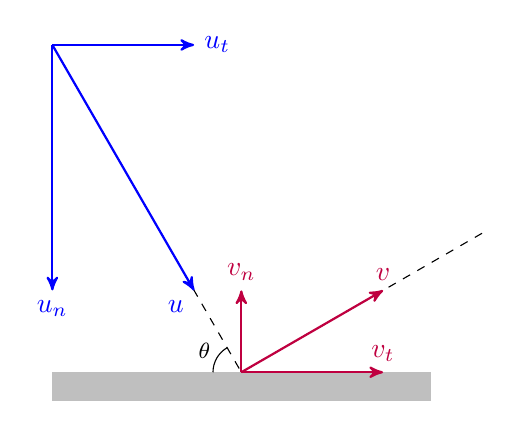
\begin{tikzpicture}[scale=1.2]
		\draw[gray!50,fill] (-2,-0.3) rectangle (2,0);
		\draw[dashed] (120:4) -- (0,0) -- (30:3);
		\draw[thick,blue,->] (120:4) --++ (-60:3) node[below left]{$u$};
		\draw[thick,purple,->] (0:0) --++ (30:1.732) node[above]{$v$};
		\draw[thick,blue,->] (120:4) --++ (1.5,0) node[right]{$u_t$};
		\draw[thick,blue,->] (120:4) --++ (0,-2.598) node[below]{$u_n$};
		\draw[thick,purple,->] (0:0) --++ (0:1.5) node[above]{$v_t$};
		\draw[thick,purple,->] (0:0) --++ (90:0.866) node[above]{$v_n$};
		\draw (120:0.3) arc(120:180:0.3);
		\node at (150:0.45) {{\footnotesize $\theta$}};
		\end{tikzpicture}
	\end{center}
\end{figure}

there is contact force normal to barrier, so there is change of momentum in this direction

change in normal component of velocity depends on coefficient of restitution

barrier is smooth, i.e., no tangential force, so no change in tangential momentum

tangential component of velocity remains unchanged after collision

components of velocity before and after collisions are: 

{

\centering

$v_t = u_t = u\cos\theta$, $\quad v_n = eu_n = eu \sin\theta$

}



\example{A sphere hits a smooth vertical barrier at $60^\circ$ to the direction of motion. In the impact with the wall, the sphere loses $\frac{2}{3}$ of its kinetic energy. Find the coefficient of
restitution between the sphere and the wall.}

components of velocity before collision are: 

{

\centering

$u_t = u\cos60^\circ = \frac{1}{2}u, \quad u_n = u\sin60^\circ = \frac{\sqrt{3}}{2}u$

}

components of velocity after collision are: 

{

\centering

$v_t = u_t = \frac{1}{2}u, \quad v_n = eu_n = \frac{\sqrt{3}}{2}eu$

$v^2 = v_t^2 + v_n^2 = \frac{1}{4}u^2 + \frac{3}{4}e^2u^2 = \frac{1+3e^2}{4}u^2$

}

$\frac{2}{3}$ of K.E. is lost, so $\frac{1}{2}mv^2 = \frac{1}{3} \cdot \frac{1}{2}mu^2$, or $v^2 = \frac{1}{3} u^2$, therefore

{
	
\centering
	
$\frac{1+3e^2}{4}u^2 = \frac{1}{3}u^2 \RA 1+3e^2 = \frac{4}{3} \RA e=\frac{1}{3}$ 
	
}


\section{Circular Motion}

\subsection{angular quantities}

position vector $\vec{r}$ $\longrightarrow$ angular displacement $\theta$

rate of change in angular displacement $\longrightarrow$ angular velocity: $\boxed{\omega = \ddt{\theta} = \dot{\theta}}$

rate of change in angular velocity $\longrightarrow$ angular acceleration: $\boxed{\alpha = \ddt{\omega} = \ddot{\theta}}$

\subsubsection*{relation to linear quantites}

distance moved out along an arc: $s=\theta r$

linear speed: $v=\ddt{s} = \ddt{(\theta r)} = \ddt{\theta} r \RA \boxed{v=\omega r}$

acceleration is a more complicated issue, we leave that for next subsection

\subsubsection*{uniform accelerated motion}

for uniformly accelerated circular motion, $\alpha = \text{const}$

angular displacement and angular velocity change with time

these are analogous to linear quantities (displacement, velocity, acceleration)

\begin{center}
	\begin{tabular}{|c|c|}
		\hline
		 uniformly accelerated linear motion & uniformly accelerated circular motion \\
		 \hline
		 $v = v_0 + a t$ & $\omega = \omega_0 + \alpha t$\\
		 $s = s_0 + v_0 t + \frac{1}{2}at^2$ & $\theta = \theta_0 + \omega_0 t + \frac{1}{2}\alpha t^2$ \\
		 $2a\Delta s = v^2 - v_0^2$	 &  $2\alpha \Delta \theta = \omega ^2 - \omega_0^2$ \\
		 \hline
	\end{tabular}
\end{center}

\subsection{acceleration}

acceleration is rate of change in velocity, which has both magnitude and direction

for linear motion, only magnitude of velocity changes, so only concept of linear acceleration

for circular motion, both magnitude and direction of velocity can change

we need two types of acceleration, responsible for changing magnitude and direction of $\vec{v}$


\begin{figure}[htp]
	\centering
\begin{minipage}{0.4\textwidth}
\begin{center}
	\begin{tikzpicture}[scale = 1.35]
	\draw[dashed] (0,0) node[below]{$O$} -- (60:5) node[below]{$A$};
	\draw[dashed] (0,0) -- (75:5) node[below left]{$B$};
	\draw[dashed] (50:5) arc(50:85:5);
	\draw[blue,thick,->] (60:5) -- ++(150:1) node[midway, above]{$\vec{v}$};
	\draw[blue,thick,->] (75:5) -- ++(165:1.8) node[midway, above]{$\vec{v}'$};
	\draw (60:1.5) arc(60:75:1.5);
	\node at (68:1.8) {$\Delta \theta$};
	\end{tikzpicture}
\end{center}
\end{minipage}\hfil
\begin{minipage}{0.4\textwidth}
	\begin{center}
		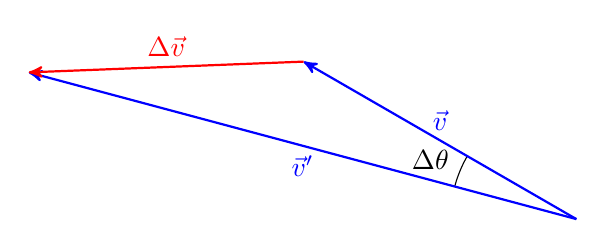
\begin{tikzpicture}[scale=4]
		\draw (150:0.4) arc(150:165:0.4);
		\node at (158:0.5) {$\Delta \theta$};
		\draw[blue,thick,->] (0:0) -- (150:1) node[midway, above]{$\vec{v}$};
		\draw[blue,thick,->] (0:0) -- (165:1.8) node[midway, below]{$\vec{v}'$};
		\draw[->,thick,red] (150:1) -- (165:1.8) node[midway, above]{$\Delta \vec{v}$};
		\end{tikzpicture}
	\end{center}

\centering
$\Downarrow$

	\begin{center}
	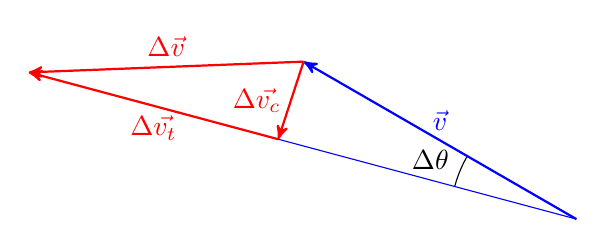
\begin{tikzpicture}[scale=4]
	\draw (150:0.4) arc(150:165:0.4);
	\node at (158:0.5) {$\Delta \theta$};
	\draw[blue,thick,->] (0:0) -- (150:1) node[midway, above]{$\vec{v}$};
	\draw[blue] (0:0) -- (165:0.98);
	\draw[->,thick,red] (150:1) -- (165:1.8) node[midway, above]{$\Delta \vec{v}$};
	\draw[->,thick,red] (150:1) -- (165:0.98) node[midway, left]{$\Delta \vec{v_c}$};
	\draw[->,thick,red] (165:0.98) -- (165:1.8) node[midway, below]{$\Delta \vec{v_t}$};
	\end{tikzpicture}
\end{center}
\end{minipage}
\end{figure}

suppose an object moves from $A$ to $B$ in short time interval $\Delta t$

change in velocity is: $\Delta \vec{v} = \vec{v}' - \vec{v}$

its acceleration: $\vec{a} = \frac{\Delta \vec{v}}{\Delta t} = \frac{\Delta \vec{v_t}}{\Delta t} + \frac{\Delta \vec{v_c}}{\Delta t}$ (see vector diagram)

as $\Delta t \to 0$, $\Delta \theta \to 0$, $\Delta \vec{v_t}$ becomes parallel to $\vec{v}$, $\Delta \vec{v_c}$ becomes normal to $\vec{v}$

so $\Delta \vec{v_t}$ gives an increase in magnitude of velocity, while $\Delta \vec{v_c}$ changes the direction

acceleration can be considered as the sum of two parts: $\boxed{\vec{a} = \vec{a_t} + \vec{a_c}}$

tangential acceleration $a_t$ (or transverse acceleration), that changes magnitude of $\vec{v}$

centripetal acceleration $a_c$ (or normal acceleration), that changes direction of $\vec{v}$

\subsubsection*{tangential acceleration}

from previous discussions, $\boxed{a_t = \ddt{v}}$

$a_t$ is closely related to angular acceleration $\alpha$: $\ddt{v} = \ddt{(\omega r)} = \ddt{\omega} r \RA \boxed{a_t = \alpha r}$ or $\boxed{a_t = \ddot{\theta} r}$

\subsubsection*{centripetal acceleration}

from vector diagram, $\Delta v_c \approx v \Delta \theta$, so $a_c = \frac{\Delta v_c}{\Delta t} \approx \frac{v \Delta \theta}{\Delta t}$

taking the limit $\Delta t \to 0$, $\omega = \ddt\theta$, so $a_c = v\omega$ $\RA$ $\boxed{a_c = \frac{v^2}{r}}$ or $\boxed{ a_c = \omega^2 r  = \dot{\theta}^2 r}$

\subsubsection*{resultant acceleration}

resultant acceleration: $\vec{a} = \vec{a_t} + \vec{a_c}$

where its magnitude is given by: $a = \sqrt{a_t^2 + a_c^2}$

\subsubsection*{vector analysis ($\star$)}

we can formally define $\vec{\omega}$ in terms of a cross product: $\boxed{\vec{v} = \vec{\omega} \times \vec{r}}$

direction of cross product is defined using the right-hand grip rule

\begin{figure}[htp]
	\centering
	\begin{tikzpicture}[scale=1.2]
	\draw (0,0) ellipse (3 and 1);
	\draw (-3,0) -- (-3,-0.1) (3,0) -- (3,-0.1);
	\draw[purple,thick,->] (0,0) node[right]{$O$} --++ (0,2.2) node[left]{$\vec{\omega}$};
	\draw[thick,->] (0,0) -- (159.54:2.134) node[above,midway]{$\vec{r}$};
	\draw[thick,->,blue] (159.54:2.134) -- ++ (200:2) node[above]{$\vec{v}$};
%	\draw[->] (0,0) --++ (-3,-2) node[left]{$x$};
%	\draw[->] (0,0) --++ (4.5,0) node[above]{$y$};
%	\draw[thick, ->] (0.16,1.5) arc(-70:250:0.45 and 0.2);
%	\draw[thick, ->] (4,0.16) arc(20:340:0.2 and 0.45);
%	\draw[thick, ->] (-2.4,-1.8) arc(-100:210:0.4 and 0.25);
	\end{tikzpicture}
\end{figure}

$\vec{a} = \ddt{\vec{v}} = \ddt{(\vec{\omega} \times \vec{r})} = \ddt{\vec{\omega}} \times \vec{r} + \vec{\omega} \times \ddt{\vec{r}} \RA \vec{a} = \vec{\alpha}\times\vec{r} + \vec{\omega}\times(\vec{\omega}\times\vec{r})$

$\vec{\alpha}\times\vec{r}$ is in tangential direction, so this is $a_t = \alpha r$

$\vec{\omega}\times(\vec{\omega}\times\vec{r})$, or $\vec{\omega}\times\vec{v}$, is in radial direction, so this is $a_c = \omega^2 r$

this reproduces the same results we obtained from vector diagrams

\example{Particle $P$ moves on an arc of a circle with centre $O$ and radius $R=0.5$ m. At time $t = 0$,	$P$ is at point $A$. At time $t$ seconds, angle $POA = t^3 - 4t$. What is its acceleration at $t=2$?}

angular velocity: $\omega = \ddt\theta = \opdt\big(t^3 - 4t\big) = 3t^2 -4$

angular acceleration: $\alpha = \ddt\omega  = \opdt\big(3t^2 -4\big)  = 6t$

at $t=2$, tangential acceleration: $a_t = \alpha R = (6\times2)\times 0.5 = 6 \mpss$

centripetal acceleration: $a_c = \omega^2 R = (3\times2^2 - 4)^2 \times 0.5 = 32\mpss$

resultant acceleration: $a = \sqrt{a_t^2 + a_c^2} = \sqrt{6^2 + 32^2} \approx 32.6\mpss$ \eoe


\subsection{force analysis}

resultant force $\vec{F} = m\vec{a}$, so it can be split into two parts $\vec{F} = \vec{F_t} + \vec{F_c}$

$\boxed{F_t = m\ddt{v}}$, or $\boxed{F_t = m r\ddot{\theta}}$, is the tangential force that changes magnitude of velocity

$\boxed{F_c = \frac{mv^2}{r}}$, or $\boxed{F_c = m \dot{\theta}^2 r}$, is the centripetal force that changes direction of motion

centripetal force is essential for circular motion

if no sufficient force to provide required $F_c$, object will not be able to follow a circular path

\vspace*{\baselineskip}

to solve a mechanics problem concerning circular motion, one could follow these guidelines

\begin{compactenum}
	\item consider energy changes and find speed of object at a particular position
	
	\item consider the forces acting (usually weight, normal reaction $N$ due to a surface, tension $T$ in a string, etc), resolve in the tangential and radial directions
	
	\item find resultant force along the radial direction, which provides centripetal force, then the equation of motion can be written down: $F_c = \frac{mv^2}{r}$ or $F_c=m\omega^2r$\footnote{Alert: the notation adopted by the A-level examination board is quite a nightmare. Instead of reserving for acceleration, the letter $a$ is often used to represent length of a string, radius of a circular track, or things like that. In this section, I use $r$ and $l$ for length quantities and save $a$ for acceleration to avoid confusion, but do watch out what the symbol $a$ means when you write down your equations.}
	
	(in some cases, equation of motion along tangential direction might also be useful)
	
	\item obtain an equation for normal reaction or tension
	
	\item look at a certain condition (object loses contact $N=0$, string becomes slack $T=0$, etc.), substitute numerical values and solve the equation
\end{compactenum}

\example{Particle $P$ is attached to one end of a light inextensible string of length $l$. The other end of the string is fixed at point $O$. Particle $P$ hangs freely below $O$, and is projected horizontally with initial speed $u$. (a) When $OP$ makes an angle $\theta$ with the downward vertical and string remains taut, what is the tension in the string? (b) If particle $P$ can complete full circle, what is the minimum initial speed needed?} \label{ex-swing}

\begin{figure}[htp]
	\centering
	\begin{minipage}{0.42\textwidth}
		\begin{center}
			\begin{tikzpicture}[scale=0.75]
			\draw[dashed] (0,0) node[above]{$O$} circle(4);
			\draw[fill] (0,-4) circle(0.08) node[above left]{$A$};
			\draw[thick,->] (-0.5,-4.3) -- ++(1,0) node[midway, below]{$u$};
			\draw[fill] (-60:4) circle(0.08) node[above]{$P$};
			\draw[dashed] (0,-3.7) -- (0,0) -- (-60:4);
			\draw[blue,thick,->] (-60:4) --++ (0,-3) node[below]{$mg$};
			\draw[purple,thick,->] (-60:4) --++ (-60:2.598) node[midway,above,rotate=-60]{{\scriptsize $mg\cos\theta$}};
			\draw[purple,thick,->] (-60:4) --++ (-150:1.5) node[midway, above, rotate=30]{{\scriptsize $mg\sin\theta$}};
			\draw[purple,dashed] (-60:6.598) --++ (-150:1.5) --++ (120:2.598);
			\draw[blue,thick,->] (-60:4.1) --++ (120:2.5) node[above]{$T$};
			\draw (-60:0.6) arc(-60:-90:0.6);
			\node at (-75:0.8) {$\theta$};
			\draw (-60:4.6) arc(-60:-90:0.6);
			\node at (-62.5:4.8) {$\theta$};
			\end{tikzpicture}
			
			Example \ref{ex-swing}
		\end{center}
	\end{minipage}\hfil
	\begin{minipage}{0.56\textwidth}
		\begin{center}
			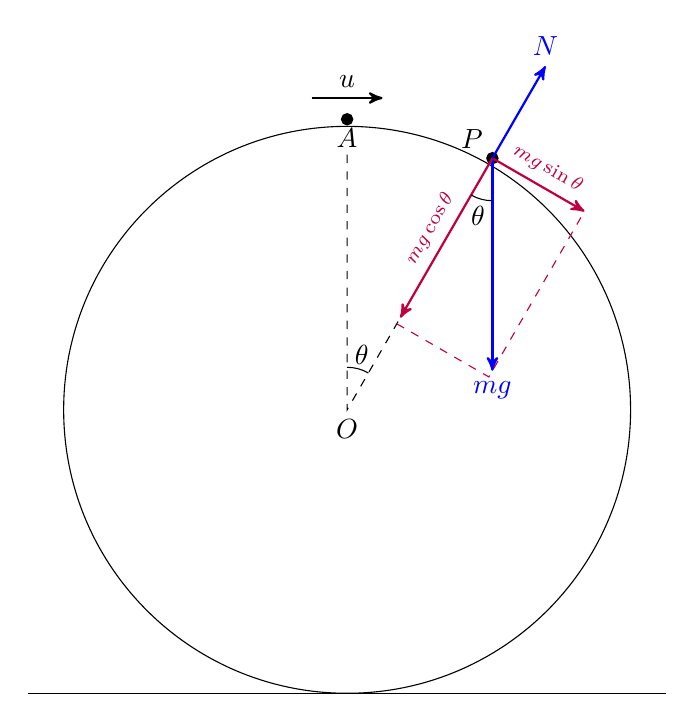
\begin{tikzpicture}[scale=0.9]
			\draw(0,0) node[below]{$O$} circle(4);
			\draw (-4.5,-4) -- (4.5,-4);
			\draw[fill] (0,4.1) circle(0.08) node[below]{$A$};
			\draw[thick,->] (-0.5,4.4) -- ++(1,0) node[midway, above]{$u$};
			\draw[fill] (60:4.1) circle(0.08) node[above left]{$P$};
			\draw[dashed] (0,3.6) -- (0,0) -- (60:4);
			\draw[blue,thick,->] (60:4.1) --++ (0,-3) node[below]{$mg$};
			\draw[purple,thick,->] (60:4.1) --++ (60:-2.598) node[midway,above,rotate=60]{{\scriptsize $mg\cos\theta$}};
			\draw[purple,thick,->] (60:4.1) --++ (-30:1.5) node[midway, above, rotate=-30]{{\scriptsize $mg\sin\theta$}};
			\draw[purple,dashed] (60:1.402) --++ (-30:1.5) --++ (60:2.598);
			\draw[blue,thick,->] (60:4.1) --++ (60:1.5) node[above]{$N$};
			\draw (60:0.6) arc(60:90:0.6);
			\node at (75:0.8) {$\theta$};
			\draw (60:3.5) arc(240:270:0.6);
			\node at (56:3.3) {$\theta$};
			\end{tikzpicture}
			
			Example \ref{ex-slidingP}
		\end{center}
	\end{minipage}
\end{figure}

from $A$ to $P$, K.E. loss = G.P.E. gain:

{\centering
	$\frac{1}{2}mu^2 - \frac{1}{2}mv^2 = mgl(1-\cos\theta)$
	
	$v^2 = u^2 - 2gl(1-\cos\theta)$
	
}

at $P$, consider the centripetal force acting:

{\centering
	$F_c = T - mg\cos\theta = \frac{mv^2}{l}$
	
	$T = mg\cos\theta + \frac{m}{l}\left(u^2 - 2gl(1-\cos\theta)\right)$
	
	$T = \frac{mu^2}{l} - mg(2 - 3\cos\theta) $
	
}

if $P$ completes full circle, string never slacks, so $T>0$ for any $\theta$

at top of circle, $\cos \theta = \cos 180^\circ = -1$, this gives minimum $T$ during the motion

{\centering
	$T_\tmin = \frac{mu^2}{l} - mg(2 + 3) > 0$
	
	$u^2 > 5gl$
	
}

minimum initial speed needed is therefore $u_\tmin = \sqrt{5gl}$ \eoe


\example{A smooth sphere of radius $R$ rests on a horizontal plane. A particle $P$ is projected horizontally with initial speed $u=\frac{1}{2}\sqrt{gR}$ from the top of the sphere and travels along the outer surface. (a) When $OP$ makes an angle $\theta$ with the upward vertical and $P$ remains in contact with the sphere, what is the normal contact force? (b) At what angle does $P$ lose contact with the sphere? (c) When the particle hits the plane, what are the horizontal and vertical components of its velocity?} \label{ex-slidingP}


from $A$ to $P$, K.E. gain = G.P.E. loss:

{\centering
$\frac{1}{2}mv^2 - \frac{1}{2}mu^2 = mgR(1-\cos\theta)$

$v^2 = u^2 + 2gR(1-\cos\theta) = \frac{1}{4}gR + 2gR(1-\cos\theta)$

$v^2 = \frac{9}{4}gR -2gR\cos\theta$

}

at $P$, consider the centripetal force acting:

{\centering
	$F_c = mg\cos\theta - N = \frac{mv^2}{R}$
	
	$N = mg\cos\theta - \frac{m}{R}\left(\frac{9}{4}gR -2gR\cos\theta\right)$
	
	$N = mg\left(3\cos\theta -\frac{9}{4}\right)$
	
}

when $P$ loses contact, contact force vanishes, i.e., $N=0$, so one has

{\centering
	$\cos\theta=\frac{3}{4} \RA \theta \approx 41.4^\circ$
	
}

after losing contact, motion only affected by gravity, so particle undergoes projectile motion

at start of projectile, the initial velocity

{\centering
	$v_0^2 = \frac{9}{4}gR - 2gR\cdot \frac{3}{4} = \frac{3}{4}gR$
	
}

horizontal component of velocity is constant, so

{\centering
	$v_x = v_{0,x} = v_0 \sin\theta \RA v_x =  \frac{\sqrt{7}}{4}\cdot \sqrt{\frac{3}{4}gR} \RA v_x = \sqrt{\frac{21gR}{64}}$
	
}

next, consider vertical motion under constant acceleration of free fall

{
	
	\centering 
	
	$v_y^2 = v_{0,y}^2 + 2gh = \left(v_0\cos\theta\right)^2 + 2g(1+\cos\theta)R = \frac{3}{4}gR\cdot \left( \frac{3}{4}\right)^2 + 2g\left(1+\frac{3}{4}\right)R \RA v_y = \sqrt{\frac{251gR}{64}} $
	
}

\example{A smooth circular hoop of radius $r$ with
	centre $O$ is fixed in a vertical plane. Two small rings $A$ and $B$, each of mass $m$, are threaded on the hoop and joined by a light inextensible string. Given that the string remains taut, $OC$ makes an angle $\theta$ with the upward vertical where $C$ is the mid-point of the string. The system is slightly displaced from its equilibrium position in
	which $\theta = 0$. At time $t$ the angle $AOB = 2\beta$. (a) By considering the total energy of the system, find an expression for the angular speed $\dot{\theta}$ of the system. (b) Find an expression for the angular acceleration $\ddot{\theta}$. (c) By considering the tangential acceleration of the rings, find the tension in the string in terms of $\theta$.} \label{ex-loopring}

\begin{figure}[htp]
	\begin{center}
		\begin{tikzpicture}[scale=1]
		\draw[thick, white, ->] (165:4) --++ (165:2.5); 
		\draw (0,0) node[below]{$O$} circle(4);
		\draw[dashed] (125:4) node[left]{$A$} -- (0,0) node[midway,below left]{$r$} -- (15:4) node[midway, below]{$r$} node[above right]{$B$};
		\draw (125:4) -- (15:4) node[midway,above]{$C$};
		\draw[dashed] (0,0) -- (70:2.294);
		\draw[very thick, rotate=125] (4,0) ellipse (0.1 and 0.05);
		\draw[very thick, rotate=15] (4,0) ellipse (0.1 and 0.05);
		\draw[dashed] (0,0) --++ (0,2);
		\draw(0,1) arc(90:70:1);
		\node at (80:1.2) {{\footnotesize $\theta$}};
		\draw(70:0.8) arc(70:15:0.8);
		\node at (42:1.1) {{\footnotesize $\beta$}};
		\draw(90:0.8) arc(90:125:0.8);
		\node at (106:1) {{\tiny $\beta-\theta$}};
		\draw[thick, blue, ->] (125:4) --++ (0,-1.8) node[left]{$mg$}; 
		\draw[thick, blue, ->] (125:4) --++ (-20:1.5) node[above]{$T$}; 
		\draw[thick, blue, ->] (125:4) --++ (125:2.5) node[above]{$N_A$}; 
		\draw[thick, blue, ->] (15:4) --++ (0,-1.8) node[left]{$mg$}; 
		\draw[thick, blue, ->] (15:4) --++ (160:1.5) node[above]{$T$}; 
		\draw[thick, blue, ->] (15:4) --++ (15:2.5) node[above]{$N_B$}; 
		\draw[dashed] (125:4) --++ (35:2);
		\draw[dashed] (125:4) --++ (215:2);
		\draw[dashed] (15:4) --++ (105:2);
		\draw[dashed] (15:4) --++ (-75:2);
		\end{tikzpicture}
		
	Example \ref{ex-loopring}
	\end{center}
\end{figure}

loss in G.P.E. for $B$ = gain in G.P.E. for $A$ + increase in K.E. for system

{

\centering

$mgr\left[\cos\beta-\cos(\beta+\theta)\right] = mgr\left[\cos(\beta-\theta) - \cos\beta\right] + 2\times\frac{1}{2}mv^2$

$v^2 = gr\left[2\cos\beta - \cos(\beta+\theta) - \cos(\beta-\theta)\right]$

}

using trigonometric identity $\cos(x\pm y) = \cos x \cos y -\mp \sin x \sin y$, we find

{

\centering

$v ^2 = gr(2\cos\beta-2\cos\beta\cos\theta) \RA v^2 = 2gr\cos\beta(1-\cos\theta)$

$\dot{\theta}^2 = \frac{v^2}{r^2} \RA \dot{\theta}^2 = \frac{2g}{r}\cos\beta(1-\cos\theta)$

}

taking time derivative of $\dot{\theta}^2$:

{

\centering

$2\dot{\theta}\cdot\ddot{\theta} = \frac{2g}{r}\cos\beta\sin\theta\cdot\dot{\theta} \RA \ddot{\theta} = \frac{g}{r}\cos\beta\sin\theta$

}

tangential motion of $A$ gives: $T\cos\beta - mg\sin(\beta-\theta) = m r\ddot{\theta}$

tangential motion of $B$ gives: $mg\sin(\beta+\theta) - T\cos\beta = m r\ddot{\theta}$

adding the two equations, one can find exactly the same result for $\ddot{\theta}$ after a bit algebra

subtracting the two equations, we obtain

{

\centering 

$2T\cos\beta = mg \sin(\beta+\theta) + mg\sin(\beta-\theta)$

}

using trigonometric identity $\sin(x\pm y) = \sin x \cos y \pm \sin x \cos y$, this simplifies to

{
	
	\centering 
	
	$2T \cos\beta = 2 mg \sin\beta \cos\theta \RA T = mg \tan\beta \cos\theta$
	
}

\section{Simple Harmonic Motion}

object moves back and forth about an equilibrium position $\longrightarrow$ oscillatory motion

must have restoring force always pointing towards equilibrium position

acceleration is in opposite direction to displacement

if magnitude of acceleration is proportional to displacement $\longrightarrow$ simple harmonics

defining equation for simple harmonic oscillation: $\boxed{a=-\omega^2x}$ or $\boxed{\dddt{x} = -\omega^2 x}$ or $\boxed{\ddot{x} = -\omega^2 x}$

\subsection{kinematic relations}

\subsubsection{displacement-time relation}

equation of motion $\dddt{x} = -\omega^2 x$ is a second-order differential equation

general solution for displacement-time relation is $\boxed{x(t) = x_0 \sin(\omega t + \phi)}$

$x_0$ is greatest value for displacement, i.e., amplitude of oscillation

$\phi$ is called the phase angle, which depends on initial conditions at $t = 0$

by choosing sine or cosine function wisely, one can avoid using the $\phi$ term

$\omega$ is called angular frequency, which is related to period of the oscillator: $\omega = \frac{2\pi}{T}$

\example{An oscillator is displaced by 4 cm from its equilibrium position and released. Given that the oscillation is simple harmonic, and period of this oscillation is 2 s. What is its displacement at $t=0.75$ s?}

angular frequency: $\omega = \frac{2\pi}{T} = \frac{2\pi}{2} = \pi \radps$

initial condition, $x(0)=x_0= 4$ cm at $t=0$

so displacement-time relation can be written as $x=x_0 \cos\omega t$

at $t=0.75$ s, $x=4\cos(\pi\times0.75) = -2\sqrt{2}$ (cm) \eoe

\subsubsection{velocity relations}

velocity-time relation: $v(t) = \ddt{x} \RA \boxed{v(t) = \omega x_0 \cos(\omega t + \phi)}$

to avoid $\phi$, again one can choose a suitable trigonometric function to fit initial conditions

taking $v^2 + (\omega x)^2$ and cancelling sines and cosines: $\boxed{v^2 = \omega^2 (x_0^2 - x^2)}$

this gives speed of oscillator at given position

maximum speed $\boxed{v_\tmax = \omega x_0}$ when $x = 0$

minimum speed $v_\tmin = 0$ when $x = \pm x_0$

\subsubsection{acceleration relations}

acceleration relations can be obtained immediately from $a=-\omega^2 x$

acceleration-time relation can be written as: $a(t) = -\omega^2 x_0 \sin(\omega t + \phi)$

maximum acceleration $\boxed{a_\tmax = \omega^2 x_0}$ at $x=\pm x_0$

minimum acceleration $a_\tmin = 0$ at $x=0$


\example{An oscillator is initially at rest. It is given an initial speed of $4 \text{ m s}^{-1}$ and starts to perform simple harmonic motion. Given that the amplitude of this oscillator is 0.80 m, when and where does its speed first becomes half of its maximum value?}

$v_\tmax = \omega_0 x_0 \RA \omega \times 0.80 = 4 \RA \omega = 5 \radps$

since $v(0)=0$ at $t=0$, so velocity-time relation is: $v(t) = v_\tmax \sin\omega t$

when $v=\frac{1}{2}v_\tmax$, then $\frac{1}{2}v_\tmax = v_\tmax \sin\omega t \RA \sin5t = \frac{1}{2} \RA t=\frac{\pi}{30} \text{ (s)}$

$v^2 = \left(\frac{1}{2}v_\tmax\right)^2 = \omega^2 (x_0^2 - x^2) \RA \frac{1}{4}\omega^2 x_0^2 = \omega^2 (x_0^2 - x^2) \RA x = \frac{\sqrt{3}}{2}x_0 \approx 0.693 \text{ (m)}$ \eoe


\example{A simple harmonic oscillator moves along a line with centre $O$. $A$, $B$ are two points on opposite side of $O$ with $OA = 4$ cm and $OB=3$ cm. The speed of the oscillator when it passes point $A$ and $B$ are $9 \text{ cm s}^{-1}$ and $12 \text{ cm s}^{-1}$  respectively.(a) What is the amplitude of this oscillation? (b) What is the period? (c) What is the time taken for the oscillator to travel from $A$ directly to $B$?}

using $v^2 = \omega^2 (x_0^2 - x^2)$, one can write

$\Bigg\{\begin{array}{l}
 \text{at }A: \text{ } 9^2 = \omega^2 (x_0^2 - 4^2) \\
 \text{at }B: \text{ } 12^2 = \omega^2 (x_0^2 - 3^2)
\end{array} \RA \frac{81}{144} = \frac{x_0^2 - 16}{x_0^2 - 9} \RA $ amplitude $x_0 = 5 \text{ (cm)}$

angular frequency $\omega = 3 \text{ (rad s$^{-1}$)}$ $\RA$ period $T=\frac{2\pi}{\omega} = \frac{2}{3} \text{ (s)}$

set $x(0)=+x_0$ when $t=0$, then displacement-time relation is $x=x_0\cos\omega t$

at $A$: $+4 = 5\cos3t_A \RA t_A \approx 0.2145 \text{ (s)}$

at $B$: $-3 = 5\cos3t_B \RA t_B \approx 0.7381 \text{ (s)}$

time taken from $A$ to $B$: $\Delta t_{AB} = t_B - t_A \approx 0.7381 - 0.2145 \approx 0.524 \text{ (s)}$ \eoe


\subsection{dynamics}

to determine whether an object undergoes simple harmonic motion, one can:

\begin{compactenum}
	\item find equilibrium position where all forces are balanced
	
	\item assume the oscillator is displaced by some arbitrary displacement $x$ from the rest position, investigate the forces acting and find their resultant $F_\text{net}$
	
	\item use $F_\text{net} = m\ddot{x}$ \footnote{The letter $a$ is now reserved for length of elastic strings, so we are going to use $\ddot{x}$ for acceleration. Thanks to Newton's dot notation for time derivatives. Yay!}to write down the equation of motion
	
	\item solve for acceleration $\ddot{x}$, and check whether it is proportional but opposite to $x$
\end{compactenum}

\example{A particle $P$ of mass $m$ moves along a horizontal line $AB$ of length $10a$. At any time $t$, the particle $P$ is acted by two  forces, $F_A = mg\left(\frac{AP}{5a}\right)^{-\frac{1}{2}}$ acting towards $A$, and $F_B = mg\left(\frac{BP}{5a}\right)^{2}$ acting towards $B$. (a) If the particle is slightly displaced from mid-point $O$ of the line $AB$, show that it moves in approximate simple harmonic motion. (b) What is the period of this oscillation?}

\begin{figure}[htp]
	\centering
	\begin{tikzpicture}[scale=1]
	\draw (0,0) node[below]{$A$} -- (10,0) node[below]{$B$} node[below,midway]{$O$} node[below,pos=0.25]{$5a$} node[below,pos=0.75]{$5a$};
	\draw[red,->] (5.8,0.1) --++ (-2.5,0) node[above]{$F_A$};
	\draw[red,->] (5.8,0.1) --++ (2,0) node[above]{$F_B$};
	\draw[fill] (5.8,0.1) circle(0.1);
	\node[below] at (5.8,0) {$P$};
	\draw[->] (3.6,-0.8) --++ (1.4,0) node[below]{$0$} --++ (0.8,0) node[below]{$x$} --++ (1.5,0) node[right]{$+$};
	\draw (5,-0.8) --++ (0,0.1) (5.8,-0.8) --++ (0,0.1);
	\end{tikzpicture}
\end{figure}

to find equilibrium position, let $F_A = F_B$:

{\centering
	
$mg\left(\frac{AP}{5a}\right)^{-\frac{1}{2}} = mg\left(\frac{BP}{5a}\right)^{2} \RA AP=BP=5a$

}

so equilibrium position at mid-point $O$ of $AB$

when $P$ is displaced by $x$ to the right of $O$, then $AP=5a+x$, $BP=5a-x$, we have:

{\centering

$F_\text{net} = F_B - F_A = mg\left(\frac{5a-x}{5a}\right)^{2} - mg\left(\frac{5a+x}{5a}\right)^{-\frac{1}{2}}$

$m\ddot{x} = mg\left(1-\frac{x}{5a}\right)^2 + mg\left(1+\frac{x}{5a}\right)^{-\frac{1}{2}}$

}

for small number $\delta \ll 1$, binomial expansion $(1+\delta)^n = 1 + n\delta + O(\delta^2) \approx 1 + n\delta$

given that displacement from $O$ is small, so $\frac{x}{a}\ll 1$, we apply the approximation

{\centering
	
	$m\ddot{x} \approx mg\left(1-2\cdot\frac{x}{5a}\right) + mg\left(1-\frac{1}{2}\cdot\frac{x}{5a}\right) \RA \ddot{x} \approx -\frac{g}{2a}x$
	
}

so motion of $P$ is approximately simple harmonic with angular frequency: $\omega = \sqrt{\frac{g}{2a}}$

period of the oscillation: $T = \frac{2\pi}{\omega} = 2\pi \sqrt{\frac{2a}{g}} $ \eoe

\subsubsection*{elastic strings}

when an elastic spring is stretched, the extension $\Delta l$ is proportional to force applied

Hooke's law for springs applies similarly to elastic strings: $T=k\Delta l$

force constant $k$ is sometimes given in terms of the modulus of elasticity: $\lambda = kl_0$

$l_0$ is natural length of the string when no force is applied

so tension in a stretched elastic string is: $\boxed{T=\frac{\lambda}{l_0}x = \frac{\lambda}{l_0}(l-l_0)}$

elastic potential energy in an elastic string is: $\boxed{E_p = \frac{1}{2}kx^2 = \frac{\lambda}{2l_0}(l-l_0)^2}$

\example{A particle $P$ of mass $m$ rests on a smooth horizontal table, and is connected to four points $A$, $B$, $C$ and $D$ by four light elastic strings, each of natural	length $a$ and modulus of elasticity $\lambda$.  $ABCD$ forms a perfect square with diagonals of length $4a$. (a) When $P$ is displaced a short distance $x$ from centre $O$ towards $C$ and released from rest, show that $P$ describes approximate simple harmonic oscillation provided higher powers of $\frac{x}{a}$ are neglected. (b) Find approximate period of this oscillatory motion.} \label{ex-fourstrings}


\begin{figure}[htp]
	\centering
	\begin{minipage}{0.56\textwidth}
		\centering
		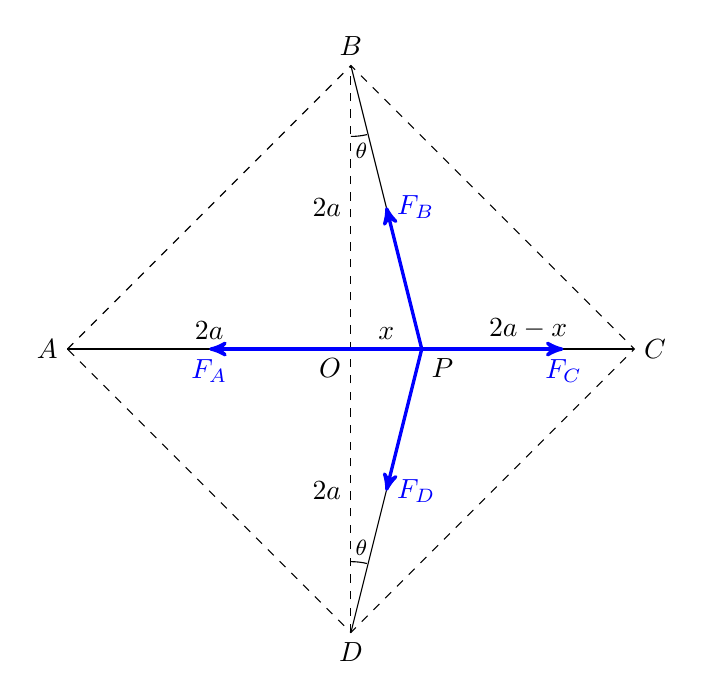
\begin{tikzpicture}[scale=.9]
		\draw[dashed] (-4,0) node[left]{$A$} -- (0,4) node[above]{$B$} -- (4,0) node[right]{$C$} -- (0,-4) node[below]{$D$} -- cycle;
		\draw (-4,0) -- (0,0) node[below left]{$O$} node[midway,above] {$2a$} -- (1,0) node[below right]{$P$} node[midway,above]{$x$} -- (4,0) node[midway,above]{$2a-x$};
		\draw (0,4) -- (1,0) -- (0,-4);
		\draw[dashed] (0,-4) -- (0,0) node[midway,left]{$2a$} -- (0,4) node[midway,left]{$2a$};
		\draw[very thick,blue,->] (1,0) -- ++(-3,0) node[below]{$F_A$};
		\draw[very thick,blue,->] (1,0) -- ++(2,0) node[below]{$F_C$};
		\draw[very thick,blue,->] (1,0) -- ++(-0.5,2) node[right]{$F_B$};
		\draw[very thick,blue,->] (1,0) -- ++(-0.5,-2) node[right]{$F_D$};
		\draw (0,3) arc(-90:-76.96:1);
		\node at (0.15,2.8) {{\footnotesize $\theta$}};
		\draw (0,-3) arc(90:76.96:1);
		\node at (0.15,-2.8) {{\footnotesize $\theta$}};
		\end{tikzpicture}
		
		Example \ref{ex-fourstrings}
	\end{minipage}\hfil
	\begin{minipage}{0.4\textwidth}
		\centering
		\begin{tikzpicture}[yscale=.9]
		\draw[fill] (0,0) node[above right]{$O$} -- (0,-5) node[right]{$N$} node[left,midway]{$a$} -- (0,-6.67) node[right]{$E$} node[left,midway]{$\frac{1}{3}a$} -- (0,-7.5) circle(0.1) node[right]{$P$} node[left,midway]{$x$};
		\draw[dashed] (0.8,-5) --++ (0.8,0) node[right,align=center,execute at begin node=\setlength{\baselineskip}{1.2em}]{{\footnotesize natural}\\ {\footnotesize position}};
		\draw[dashed] (-0.9,-6.67) --++ (0.5,0) (0.8,-6.67) --++ (0.8,0) node[right,align=center,execute at begin node=\setlength{\baselineskip}{1.2em}]{{\footnotesize equilibrium}\\ {\footnotesize position}};
		\draw[dashed] (-0.9,-7.5) --++ (0.5,0);
		\draw (-0.5,0) -- (0.5,0);
		\draw[->] (-1.2,-5) -- (-1.2,-6.67) node[left]{$0$} -- (-1.2,-7.5) node[left]{$x$} -- (-1.2,-8) node[below]{$+$};
		\draw (-1.2,-6.67) --++ (0.1,0) (-1.2,-7.5) --++ (0.1,0);
		\end{tikzpicture}
		
		Example \ref{ex-elabounce}
	\end{minipage}
\end{figure}

magnitude of resultant of $F_A$ and $F_C$ is:

{
	
	\centering
	
	$F_{AC} = F_A - F_C = \frac{\lambda}{a}(2a+x-a) - \frac{\lambda}{a}(2a-x-a) = \frac{2\lambda}{a}x$
	
}

magnitude of resultant of $F_B$ and $F_D$ is:

{
	
	\centering
	
	$F_{BD} = F_B\sin\theta + F_D\sin\theta = 2\cdot\frac{\lambda}{a}\left(\sqrt{(2a)^2+x^2} - a\right)\cdot \frac{x}{\sqrt{(2a)^2+x^2}}$
	
	\vspace*{0.1\baselineskip}
	
	$F_{BD} = \frac{2\lambda x}{a} \left(1 - \frac{a}{\sqrt{4a^2+x^2}}\right) =  \frac{2\lambda x}{a} \left\{1 - \frac{1}{2} \cdot \left(1 + \frac{x^2}{4a^2}\right)^{-\sfrac{1}{2}} \right\} $
	
}

recall binomial expansion approximation $(1+\delta)^n \approx 1 + n\delta$ for $\delta \ll 1$

given that $x \ll a$, i.e., $\frac{x}{a} \ll 1$, so one has: $\left(1 + \frac{x^2}{4a^2}\right)^{-\sfrac{1}{2}} \approx 1 -\frac{1}{2}\cdot \frac{x^2}{4a^2} $

neglecting higher powers of $\frac{x}{a}$, we find

{
	
	\centering
	
	$F_{BD} \approx \frac{2\lambda x}{a} \left(1 - \frac{1}{2} \cdot 1\right)  \RA F_{BD} \approx \frac{\lambda}{a}x$
	
}

now consider the resultant force, also note that both $F_{AC}$ and $F_{BD}$ act to the left, so

{
	
	\centering
	
	$F_\text{net} = -F_{AC} - F_{BD} \RA m\ddot{x} = -\frac{2\lambda}{a}x - \frac{\lambda}{a}x \RA \ddot{x} = -\frac{3\lambda}{ma}x $
	
}

hence particle $P$ describes simple harmonic oscillation with period $T=\frac{2\pi}{\omega} = 2\pi\sqrt{\frac{ma}{3\lambda}}$ \eoe


\example{A particle of mass $m$ is suspended at the end of an elastic cord of natural length $a$ and modulus of elasticity $3mg$. The particle is released from rest from $\frac{1}{4}a$ above the equilibrium position. (a) Show that the particle will perform simple harmonic motion. (b) Find the greatest speed during the oscillation. (c) Find when the particle first reach this maximum speed.} \label{ex-elabounce}

equilibrium when $mg=\frac{\lambda}{a}\Delta l =\frac{3mg}{a}\Delta l \RA \Delta l = \frac{1}{3}a$

so equilibrium position $E$ at $\frac{1}{3}a$ below natural position

take positive direction as vertically downwards

when particle is displaced by $x$: $F_\text{net}=mg-T = mg - \frac{\lambda}{a}\Delta l$

{
\centering

$m\ddot{x} = mg - \frac{3mg}{a} \left(\frac{1}{3}a+x\right) \RA \ddot{x} = - \frac{3g}{a}x$

}

so simple harmonics with angular frequency $\omega =\sqrt{ \frac{3g}{a}}$

at $t=0$, initial position $x(0)=-\frac{1}{4}a$, amplitude is magnitude of initial displacement $x_0 = \frac{1}{4}a$

maximum speed $v_\tmax = \omega x_0 = \sqrt{ \frac{3g}{a}} \cdot \frac{1}{4}a \RA v_\tmax = \frac{\sqrt{3ga}}{4}$

at $t=0$, $v(0)=0$, particle starts to move downwards (positive direction)

so can write down velocity-time relation: $v(t) = v_\tmax \sin \omega t$

greatest speed when $\sin\omega t=1$, or $\omega t = \frac{\pi}{2} \RA t= \frac{\pi}{2}\sqrt{\frac{a}{3g}}$ 

alternatively, note that speed becomes maximum when particle passes equilibrium position

this completes one quarter of a full oscillation, which takes $\frac{1}{4}$ of one period

so time taken to reach $v_\tmax$ is: $t=\frac{1}{4}T = \frac{1}{4}\cdot\frac{2\pi}{\omega} \RA  t=\frac{\pi}{2}\sqrt{\frac{a}{3g}}$  \eoe

\example{Consider the same oscillatory system in Example \ref{ex-elabounce}. If the particle is brought to a position where the length of the elastic string is $2a$ and released from rest. Find the distance $OP$ when particle $P$ reaches the greatest height, and also find the time taken for $P$ first comes to this height.}

when string remains taut, $P$ performs simple harmonic motion

we have found equilibrium is at $\frac{1}{3}a$ below natural position, and angular frequency $\omega=\sqrt{\frac{3g}{a}}$

amplitude of this oscillation: $x_0 = 2a - a -\frac{1}{3}a \RA x_0 = \frac{2}{3}a$

at $t=0$, initial displacement $x(0)=+x_0$, so displacement-time relation is: $x=x_0\cos\omega t$

when string becomes slack, string is at natural length, $x=-\frac{1}{3}a$, so

{

\centering

$v^2 = \omega^2 (x_0^2 - x^2) \RA v^2 = \frac{3g}{a} \left( \frac{4}{9}a^2 - \frac{1}{9}a^2 \right) \RA v=\sqrt{ga}$

$-\frac{1}{3}a = \frac{2}{3}a\cos\omega t_1 \RA \omega t_1 = \frac{2\pi}{3} \RA t_1 = \frac{2\pi}{3}\sqrt{\frac{a}{3g}}$

}

afterwards, no tension acts, $P$ is acted by gravity only, so constant acceleration of free fall

instantaneous speed becomes zero at highest point, so we have:

{

\centering

$0^2 - v^2 = 2\cdot(-g) \cdot \Delta h \RA \Delta h = \frac{v^2}{2g} = \frac{ga}{2g} \RA \Delta h = \frac{1}{2}a$

$0 - v = (-g)\cdot t_2 \RA t_2 = \frac{v}{g} = \frac{\sqrt{ga}}{g} \RA t_2 = \sqrt{\frac{a}{g}}$

}

hence greatest height is $\frac{1}{2}a$ above natural position of the string $\RA OP=a-\frac{1}{2}a=\frac{1}{2}a$

alternatively, one can also consider energy changes: elastic P.E. in string = G.P.E. gain

{

\centering

$\frac{1}{2}\cdot\frac{3mg}{a}\cdot(2a-a)^2 = mg\Delta H \RA \Delta H = \frac{3}{2}a$

}

this shows the greatest height is $\frac{3}{2}a$ above the point of release $\RA OP=2a-\frac{3}{2}a = \frac{1}{2}a$

total time taken $t=t_1+t_2 = \frac{2\pi}{3}\sqrt{\frac{a}{3g}} + \sqrt{\frac{a}{g}} \RA t = \left(\frac{2\pi}{3\sqrt{3}} + 1\right)\sqrt{\frac{a}{g}}$ \eoe



\section{Rotational Mechanics}

\subsection{torque}


we define torque of a force as product of force and its lever arm: $\boxed{\tau = F r}$

where lever arm $r$ is perpendicular distance from line of action to pivot

torque acting on a rigid body produces turning effects

torque is a vector quantity\footnote{More formally, torque is defined as $\vec{\tau} = \vec{r} \times \vec{F}$.}, which can act in clockwise or counter-clockwise direction


\subsubsection*{torque due to weight}

for a body of mass $M$, weight acts on every small constituent piece $\Delta m_i$, where $M=\sum_i \Delta m_i$

net torque due to weight is $\tau—_\text{body} = \sum_i \tau_i = \left(\sum_i \Delta m_i g r_i\right) = \left(\sum_i \Delta m_i r_i\right) g$\footnote{I am a bit sloppy here. We should use the lever arm distance from a chosen pivot, or we should write $\vec{\tau}_\text{body}\ = \sum_i \Delta m_i \vec{r}_i \times \vec{g}$. But as long as we keep that in mind, the results that follow are valid.}

we introduce centre of mass, such that $\boxed{\left(\sum_i \Delta m_i r_i\right) = \left(\sum_i \Delta m_i\right) r_\text{cm}}$, or $\left(\sum_i \Delta m_i r_i\right) = M r_\text{cm}$

$r_\text{cm} = \frac{\sum_i \Delta m_i r_i}{\sum_i \Delta m_i}$ gives position of centre of mass from a chosen origin

taking continuum limit: $\Delta m_i \to \dd m \RA \boxed{r_\text{cm} = \frac{\int r \dd m}{\int \dd m}}$

$r_\text{cm}$ can be thought as the weighted average of position vector $r_i$'s

net torque due to weight can be therefore computed as: $\boxed{\tau_\text{body} = Mgr_\text{cm}}$

entire weight on rigid body can be considered to act at centre of mass

\example{A uniform rod $AB$ has mass $4m$ and length $L$. A particle of mass $m$ is attached at $A$ and another particle of mass $2m$ is attached at $B$. The system is allowed to rotate about a horizontal axis perpendicular to the rod and through $A$. (a) Find the position of the centre of mass. (b) When the system is displaced by an angle $\theta$ from the downward vertical, what is the torque by gravity?} \label{ex-lever}

\begin{figure}[htp]
	\centering
	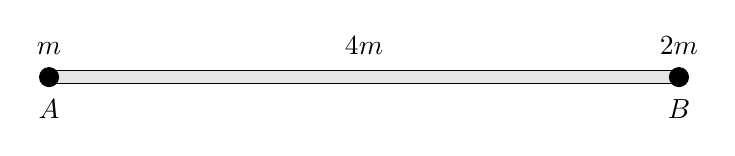
\begin{tikzpicture}[scale=0.8]
	\draw[fill=gray!20] (-5,-0.1) rectangle (5,0.1);
	\draw[fill] (-5,0) circle(0.15);
	\draw[fill] (5,0) circle(0.15);
	\node[below] at (-5,-0.2) {$A$};
	\node[below] at (5,-0.2) {$B$};
	\node[above] at (-5,0.2) {$m$};
	\node[above] at (5,0.2) {$2m$};
	\node[above] at (0,0.2) {$4m$};
	\end{tikzpicture}
	
	Example \ref{ex-lever}
\end{figure}

{
	
\centering
	
$(m\cdot 0 + 2m\cdot L + 4m \cdot \frac{1}{2}L) = (m+2m+4m)x_\text{cm} \RA x_\text{cm} = \frac{4}{7}L$

}

centre of mass is at $\frac{4}{7}L$ from $A$ (near mid-point of $AB$ but slightly closer to the heavier end)

when suspended, torque by gravity can be found using $r_\text{cm}$

{
	
\centering

$\tau = Mgr_\text{cm} \RA \tau_\text{body} = 7mg\cdot \frac{4}{7}L\sin\theta = 4mgL\sin\theta$

}

(or by summing up torques of each part: $\tau = 0 + 2mg\cdot L\sin\theta + 4mg\cdot\frac{1}{2}L\sin\theta = 4mgL\sin\theta$) \eoe

\subsection{moment of inertia}

\subsubsection{moment of inertia: the motivation}\label{moim}

a rigid body means an object never undergoes change in shape

let's think of it a system of many small pieces of mass $\Delta m_i$

distance between any two pieces remains the same whatever you do

if each piece is acted by some resultant force $F_i = \Delta m_i a_i$

torque on this piece: $\tau_i = F_i r_i = (\Delta m_i a_i) r_i = (r_i^2 \Delta m_i)\frac{a_i}{r_i}$

recall $\alpha = \frac{a_i}{r_i}$ gives the angular acceleration

torque on one individual piece: $ \tau_i =  r_i^2 \Delta m_i  \alpha $

to find out what resultant torque does, sum up for all pieces: $\sum_i \tau_i = \sum_i (r_i^2 \Delta m_i \alpha)$

but angular acceleration is the same throughout a rigid body (rotation as a whole)

so $\alpha$ can be taken out from the summation: $ \sum_i \tau_i = \left(\sum_i r_i^2 \Delta m_i\right) \alpha$

\vspace*{\baselineskip}

we introduce moment of inertia of a rigid body: $\boxed{I = \sum_i r_i^2 \Delta m_i}$

taking continuum limit: $\Delta m_i \to \dd m \RA \boxed{I = \int r^2 \dd m}$

hence we have the equivalent of Newton's $2^\text{nd}$ law: $\boxed{\sum \tau_i = I \alpha}$

this states a resultant torque on a rigid body produces angular acceleration that is inversely proportional to its moment of inertia (compare with this: a resultant force produces linear acceleration that is inversely proportional to object's inertia mass)

moment of inertia describes how a rigid body resists change in rotational motion when acted by a resultant torque, hence plays an important role in rotational mechanics

we will next study how to compute moment of inertia for different bodies

\subsubsection{moment of inertia: some useful results}

we here present the moment of inertia of some regular objects 

note that all $I$'s listed below are about a perpendicular axis through centre

\begin{center}
	{\renewcommand{\arraystretch}{1.2}
	\renewcommand{\tabcolsep}{0.2cm}
	\begin{tabular}{|cc|c|}
		\hline
		\multicolumn{2}{|c|}{uniform object with mass $m$} & moment of inertia \\
		\hline
		ring & radius $R$ & $I=mR^2$ \\ \hline
		disc/solid cylinder & radius $R$ & $I=\frac{1}{2}mR^2$ \\ \hline
		thin rod & length $2L$ & $I=\frac{1}{3}mL^2$ \\ \hline	
		rectangular lamina & sides $2a$, $2b$ & $I=\frac{1}{3}m(a+b)^2$ \\ \hline
		solid sphere & radius $R$ & $I=\frac{2}{5}mR^2$ \\ \hline
		spherical shell & radius $R$ & $I=\frac{2}{3}mR^2$ \\ \hline
	\end{tabular}}
\end{center}

all of these can be shown using the defining equation: $I = \sum_i r_i^2 \Delta m_i$, or $I = \int r^2 \dd m$

we show the proofs for a few items on the list, the rest will be left as exercise for the reader \footnote{Spoiler alert: this left-as-exercise nonsense occurs whenever the author simply does not want to typeset more equations or diagrams.}

\subsubsection*{point mass}

consider a particle of mass $m$ rotates about an axis at distance $R$

simply recall defining equation: $I_\text{pt}=mR^2$

\subsubsection*{uniform ring}

\begin{figure}[htp]
	\centering
	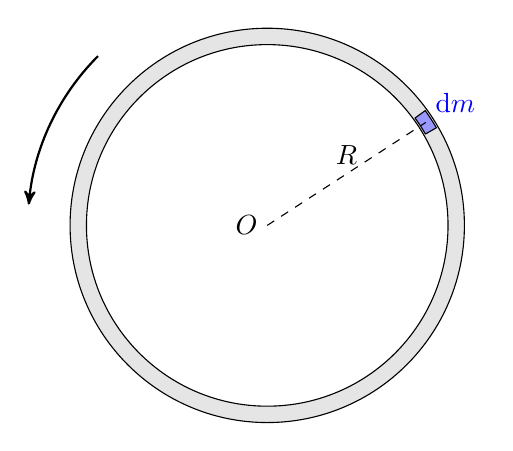
\begin{tikzpicture}[scale=0.8]
	\draw[line width=6,gray!20] (0,0) circle(3);
	\draw (0,0) circle(3.13);
	\draw (0,0) circle(2.87);
	\draw[fill=blue!40] (30:2.9) -- ++ (30:0.2) arc(30:36:3.1) --++ (36:-0.2) arc(36:30:2.9);
	\draw[dashed] (0,0)node[left]{$O$} -- (33:3) node[midway,above]{$R$} node[above right,blue]{$\dd m$};
	\draw[thick, ->] (135:3.8) arc(135:175:3.8);
	\end{tikzpicture}
	
	uniform ring of radius $R$
\end{figure}

a uniform ring of mass $m$ rotates about perpendicular axis through its centre $O$

any piece $\Delta m$ is of same distance to $O$, which is radius $R$ of the ring

so $I_\text{ring} = \int r^2 \dd m = R^2 \int \dd m \RA \boxed{I_\text{ring} = mR^2}$


\subsubsection*{uniform disc}

\begin{figure}[htp]
	\centering
	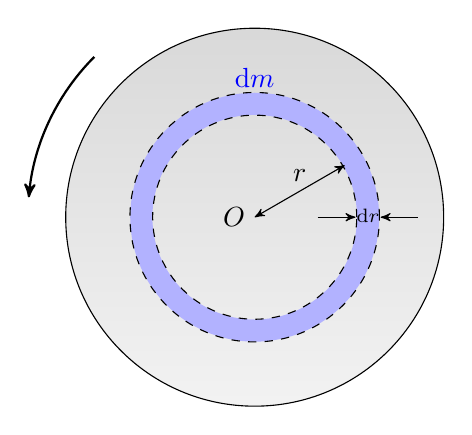
\begin{tikzpicture}[scale=0.8]
	\shadedraw[top color=gray!30,bottom color=gray!10, draw=black] (0,0) circle(3);
	\draw[line width=8,blue!30] (0,0) circle(1.8);
	\draw[dashed] (0,0) circle(1.98);
	\draw[dashed] (0,0) circle(1.62);
	\draw[<->] (0,0)node[left]{$O$} -- (30:1.65) node[midway,above]{$r$};
	\draw[->] (1,0) -- (1.6,0);
	\draw[<-] (2,0) -- (2.6,0);
	\node at (1.8,0.02) {{\scriptsize $\dd r$}};
	\node[above,blue] at (0,1.9) {$\dd m$};
	\draw[thick, ->] (135:3.6) arc(135:175:3.6);
	\end{tikzpicture}
	
	uniform disc of radius $R$
\end{figure}

a uniform disc of mass $m$ rotates about perpendicular axis through its centre $O$

consider a narrow ring of radius $r$ and thickness $\dd r$ about $O$

area of this ring is: $\dd A = 2 \pi r \dd r$

its mass is therefore: $\dd m = \frac{2 \pi r \dd r}{\pi R^2}\cdot m = \frac{2mr}{R^2}\dd r$

so $I_\text{disc} = \int r^2 \dd m = \int_0^R r^2 \frac{2mr}{R^2}\dd r = \frac{2m}{R^2}\int_0^R r^3 \dd r = \frac{2m}{R^2} \times \frac{R^4}{4}\RA \boxed{I_\text{disc} = \frac{1}{2}mR^2}$

\subsubsection*{uniform rod}

\begin{figure}[htp]
	\centering
	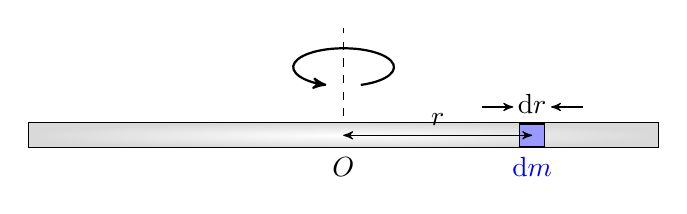
\begin{tikzpicture}[scale=0.8]
	\shadedraw[inner color=white,outer color=gray!30, draw=black] (-5,-0.2) rectangle (5,0.2);
	\draw[fill=blue!40] (2.8,-0.18) rectangle (3.2,0.18);
	\draw[<->] (0,0) -- (3,0) node[midway,above]{$r$};
	\draw[->] (2.2,0.45) -- (2.7,0.45);
	\draw[<-] (3.3,0.45) -- (3.8,0.45);
	\node at (3,0.5) {$\dd r$};
	\node[below] at (0,-0.2) {$O$};
	\node[below,blue] at (3,-0.2) {$\dd m$};
	\draw[thick, ->] (0.28,0.8) arc(-70:250:0.8 and 0.3);
	\draw[dashed] (0,0.3) --++ (0,1.4);
	\end{tikzpicture}
	
	uniform rod of length $2L$
\end{figure}

a uniform rod of mass $m$ rotates about perpendicular axis through its centre $O$

consider a narrow piece of thickness $ \dd r$ at distance $r$ from $O$

mass of this piece: $\dd m = \frac{\dd r}{2L}\cdot m = \frac{m}{2L}\dd r$

so $I_\text{rod} = \int r^2 \dd m = \int_{-L}^L r^2 \frac{m}{2L}\dd r = \frac{m}{2L} \int_{-L}^L r^2 \dd r = \frac{m}{2L} \times \frac{2L^3}{3}\RA \boxed{I_\text{rod} = \frac{1}{3}mL^2}$

\subsubsection{parallel axis theorem}

\noindent\textbf{theorem:} moment of inertia of a rigid body of mass $m$ about any axis can be found from its moment of inertia about a parallel axis through its centre of mass: $\boxed{I_P = I_\text{cm}+ md^2}$, where $d$ is perpendicular distance between the two parallel axes

\begin{figure}[htp]
	\centering
	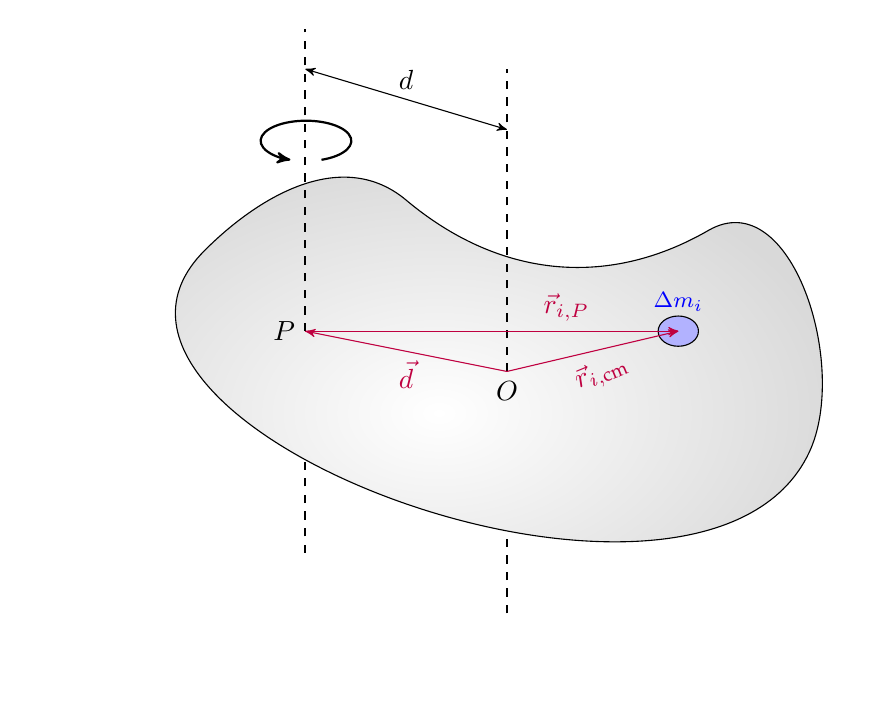
\begin{tikzpicture}[scale=1.28]
	\shadedraw[inner color=white,outer color=gray!30, draw=black] (-2,0) to [out=45,in=140] (0,0.5) to [out=-40,in=210] (3,0.2) to [out=30,in=65] (4,-2) to [out=245,in=225] (-2,0);
	\draw[dashed,thick] (1,-3.6) -- (1,-2.8) (1,-1.2)node[below]{$O$} -- ++(0,3);
	\draw[dashed,thick] (-1,-3) -- (-1,-2.1) (-1,-0.8)node[left]{$P$} -- ++(0,3);
	\draw[<->] (-1,1.8) --++ (2,-0.6) node[above,midway]{$d$};
	\draw[fill=blue!30] (2.7,-0.8) ellipse (0.2 and 0.15);
	\node[blue,above] at (2.7,-0.7) {{\footnotesize $\Delta m_i$}};
	\draw[->,purple] (-1,-0.8) -- (2.7,-0.8) node[above,pos=0.7]{$\vec{r}_{i,P}$};
	\draw[->,purple] (1,-1.2) -- (2.7,-0.8) node[below,pos=0.5,rotate=22.4]{$\vec{r}_{i,\text{cm}}$};
	\draw[<-,purple] (-1,-0.8) -- (1,-1.2) node[below,midway]{$\vec{d}$};
	\draw[thick, ->] (-.84,0.9) arc(-70:250:0.45 and 0.2);
	\end{tikzpicture}
\end{figure}

\vspace*{-\baselineskip}

\noindent\textbf{proof:} $I_P = \sum r_{i,P}^2 \Delta m_i = \sum (\vec{r}_{i,\text{cm}}-\vec{d})^2 \Delta m_i = \sum r_{i,\text{cm}}^2 \Delta m_i + \sum d^2 \Delta m_i - 2\sum \vec{r}_{i,\text{cm}} \cdot \vec{d} \Delta m_i$

first term: $I_\text{cm} = \sum r_{i,\text{cm}}^2 \Delta m_i$, so this is just moment of inertia about centre of mass

second term: $\sum d^2 \Delta m_i = d^2 \sum m_i = md^2$

in last term, we have: $\sum \vec{r}_{i,\text{cm}} \cdot \vec{d} \Delta m_i = \big(\sum \vec{r}_{i,\text{cm}} \Delta m_i \big) \cdot \vec{d}$

notice the term in bracket is related to distance from centre of mass (recall $m\vec{r}_\text{cm} = \sum \Delta m_i \vec{r}_i$)

but here we are evaluating the distance from centre of mass to centre of mass, so it is zero

put everything together, we find: $I_P = I_\text{cm}+ md^2$

\newpage

\vspace*{-1.2\baselineskip}

\example{A system consists of a solid sphere of mass $5m$ and radius $a$, a uniform rod of mass $4m$ and length $3a$ and a particle of mass $2m$. The objects are joined together as shown in the figure below. What is the moment of inertia of this system about an axis through $X$ perpendicular to the rod?} \label{ex-lollipop}

\begin{figure}[ht]
	\centering
	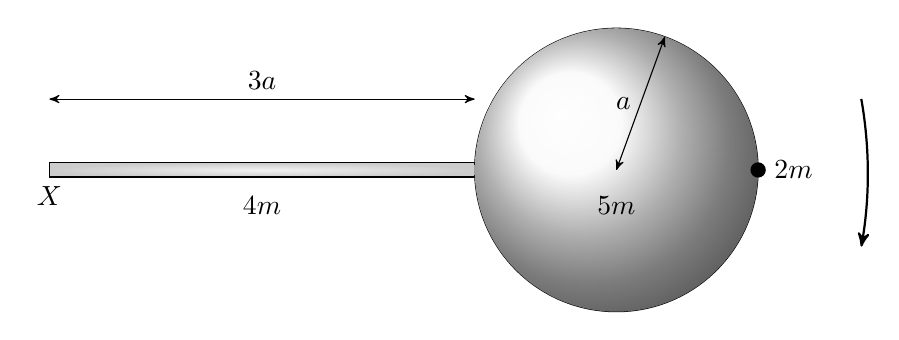
\begin{tikzpicture}[scale=0.9]
	\shadedraw[inner color=gray!10, outer color=gray!40, draw=black] (0,-0.1) node[below]{$X$} rectangle (6,0.1);
	\draw (8,0) circle (2);
	\shade[ball color = gray!5] (8,0) circle (2);
	\draw[fill] (10,0) circle(0.1);
	\draw[<->] (0,1) --++ (6,0) node[midway,above]{$3a$};
	\draw[<->] (8,0) --++ (70:2) node[midway,left]{$a$};
	\node at (3,-0.5) {$4m$};
	\node at (8,-0.5) {$5m$};
	\node at (10.5,0) {$2m$};
	\draw[thick, ->] (5:11.5) arc(10:-10:6);
	\end{tikzpicture}
%	
%	Example \ref{ex-lollipop}
\end{figure}

$I_\text{rod} = \frac{1}{3}\cdot 4m \cdot \left(\frac{3a}{2}\right)^2 + 4m \cdot \left(\frac{3a}{2}\right)^2 = (3+9) ma^2 = 12ma^2$

$I_\text{sphere} = \frac{2}{5}\cdot 5m\cdot a^2 + 5m \cdot(a+3a)^2 = (2+80) ma^2 = 82ma^2$

$I_\text{pt} = 2m \cdot (3a+2a)^2 = 50 ma^2$

$I_\text{sys} = I_\text{rod}  + I_\text{sphere}  + I_\text{pt} = (12+82+50)ma^2 \RA I_\text{sys} = 144ma^2 $ \eoe

\subsubsection{perpendicular axis theorem}

\noindent\textbf{theorem:} given a thin lamina (negligible thickness), its moment of inertia about an axis perpendicular to the plane is equal to the sum of moments of inertia about two perpendicular axes lying within the plane through the same point

suppose the lamina lies within $xy-$plane, then the theorem suggests: $\boxed{I_z = I_x + I_y}$

\begin{figure}[htp]
	\centering
	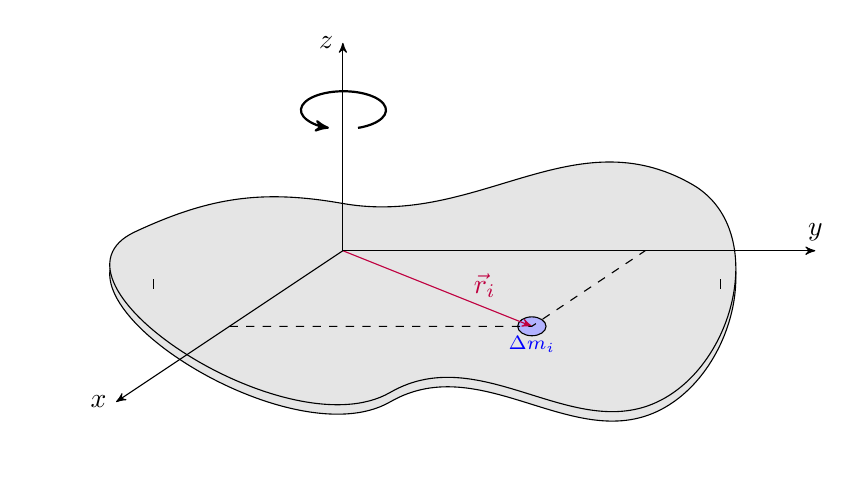
\begin{tikzpicture}[scale=1.2]
	\draw[fill=gray!20] (-3.2,0.4) to [out=25,in=170] (-1,0.7) to [out=-10,in=150] (2.7,0.9) to [out=-30,in=35] (2.5,-1.3) to [out=215,in=30] (-0.5,-1.3) to [out=210,in=205] (-3.2,0.4);
	\draw[fill=gray!20] (-3.2,0.5) to [out=25,in=170] (-1,0.8) to [out=-10,in=150] (2.7,1) to [out=-30,in=35] (2.5,-1.2) to [out=215,in=30] (-0.5,-1.2) to [out=210,in=205] (-3.2,0.5);
	\draw (-3,0) -- (-3,-0.1) (3,0) -- (3,-0.1);
	\draw[fill=blue!30] (1,-0.5) ellipse (0.15 and 0.1);
	\draw[purple,->] (-1,0.3) -- (1,-0.5) node[pos=.75,above]{$\vec{r}_i$};
	\node[blue,below] at (1,-0.5) {{\scriptsize $\Delta m_i$}};
	\draw[->] (-1,0.3) --++ (0,2.2) node[left]{$z$};
	\draw[->] (-1,0.3) --++ (-2.4,-1.6) node[left]{$x$};
	\draw[->] (-1,0.3) --++ (5,0) node[above]{$y$};
	\draw[dashed] (-2.2,-0.5) -- (1,-0.5) -- (2.2,0.3);
	\draw[thick, ->] (-.84,1.6) arc(-70:250:0.45 and 0.2);
	\end{tikzpicture}
\end{figure}

\noindent\textbf{proof:} $I_z = \sum r_{i,z}^2 \Delta m_i = \sum (x_i^2 + y_i^2) \Delta m_i$

$I_x = \sum r_{i,x}^2 \Delta m_i = \sum (y_i^2 + z_i^2) \Delta m_i$, $I_y = \sum r_{i,y}^2 \Delta m_i = \sum (x_i^2 + z_i^2) \Delta m_i$

but all $z_i \approx 0$ for thin lamina, so $I_x = \sum y_i^2 \Delta m_i$, $I_y = \sum x_i^2 \Delta m_i$

it is now obvious to see: $I_z = I_x + I_y$

\example{What is the moment of inertia of a uniform disc of radius $R$ about its diameter?}

\begin{figure}[htp]
	\centering
	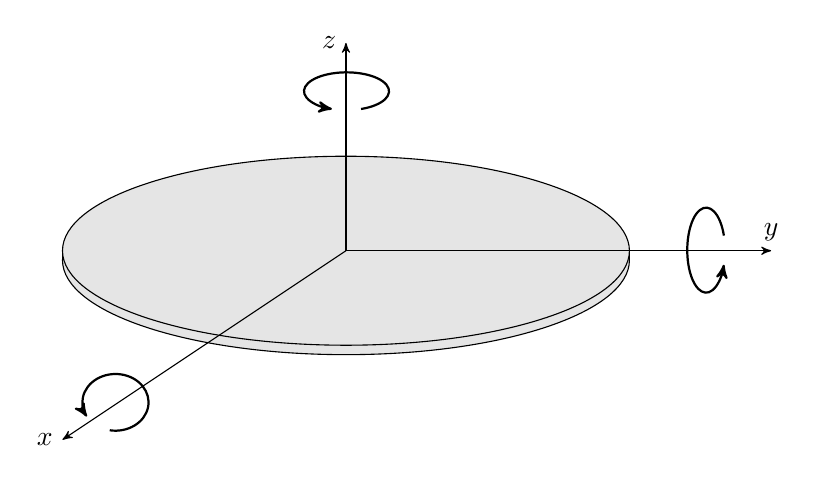
\begin{tikzpicture}[scale=1.2]
	\draw[fill=gray!20] (0,-0.1) ellipse (3 and 1);
	\draw[fill=gray!20] (0,0) ellipse (3 and 1);
	\draw (-3,0) -- (-3,-0.1) (3,0) -- (3,-0.1);
	\draw[->] (0,0) --++ (0,2.2) node[left]{$z$};
	\draw[->] (0,0) --++ (-3,-2) node[left]{$x$};
	\draw[->] (0,0) --++ (4.5,0) node[above]{$y$};
	\draw[thick, ->] (0.16,1.5) arc(-70:250:0.45 and 0.2);
	\draw[thick, ->] (4,0.16) arc(20:340:0.2 and 0.45);
	\draw[thick, ->] (-2.5,-1.9) arc(-100:210:0.35 and 0.3);
	\end{tikzpicture}
\end{figure}

set up perpendicular axes through centre of disc as shown, by theorem: $I_z = I_x + I_y$

but also due to symmetry: $I_x = I_y$, so $I_x = I_y = \frac{1}{2}I_z = \frac{1}{2}\times\frac{1}{2}mR^2 \RA I_x = I_y = \frac{1}{4}mR^2$ \eoe


\subsection{force analysis}

from last section, we have learned how to compute moment of inertia of a rigid body

also from discussion in \S \ref{moim}, we have $\sum \tau_i = I \alpha$, or $\sum \tau_i = I \ddot{\theta}$

now we can predict the motion of a rigid body by applying the equation of motion

\example{A solid cylinder of mass $M$ and radius $R$ rolls down an inclined slope without slipping. What is the acceleration of the body?} \label{ex-rolling}

\begin{figure}[htp]
	\begin{center}
		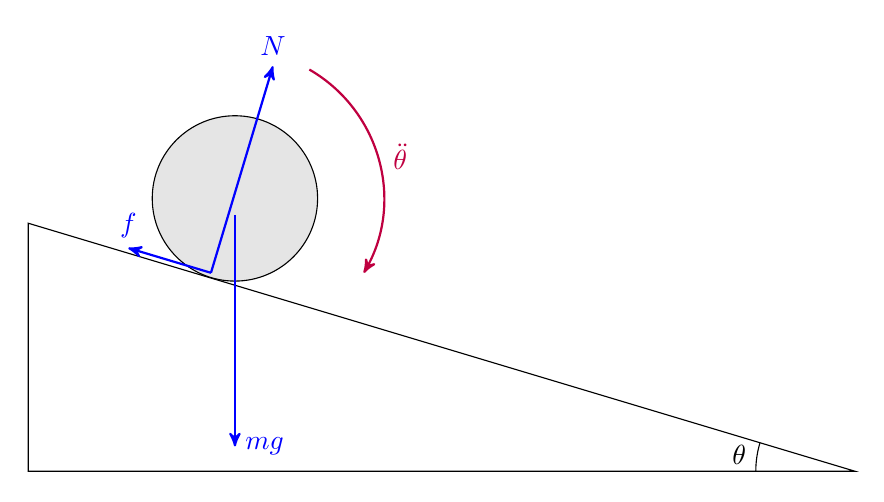
\begin{tikzpicture}[scale=1.05]
		\draw (0,0) --++ (0,3) -- (10,0) -- cycle;
		\draw[fill=gray!20] (2.5,3.3) circle (1);
		\draw[purple,->,thick] (2.5,3.3) ++ (60:1.8) arc(60:-30:1.8);
		\node[purple] at (4.5,3.8) {$\ddot{\theta}$};
		\draw[thick,blue,->] (2.5,3.1) --++ (0,-2.8) node[right]{$mg$};
		\draw[thick,blue,->] (2.21,2.4) --++ (0.75,2.5) node[above]{$N$};
		\draw[thick,blue,->] (2.21,2.4) --++ (-1,0.3) node[above]{$f$};
		\draw (8.8,0) arc(180:163.3:1.2);
		\node at (8.6,0.2) {$\theta$};
		\end{tikzpicture}
		%Example \ref{ex-rolling}
	\end{center}
\end{figure}

resolve along the slope: $mg\sin\theta - f = m\ddot{x}$

torque on cylinder: $f R = \frac{1}{2}mR^2 \cdot \ddot{\theta} \RA f = \frac{1}{2} mR\ddot{\theta}$

together with $\ddot{x}=\ddot{\theta} R$, we have: $mg\sin\theta - \frac{1}{2} mR\cdot \frac{\ddot{x}}{R} = m\ddot{x} \RA \ddot{x}=\frac{2}{3}g\sin\theta$ \eoe

\example{A uniform disc of radius $R$ and mass $M$ is free to rotate without friction about a horizontal
	axis through its centre $O$. A light inextensible string is wound round	the rim of the disc, while a particle of mass $m$ is attached to one end of the string (see diagram). The system is released from rest. Find the angular acceleration of the disc.}\label{ex-rotdisc}

\begin{figure}[htp]
	\begin{center}
		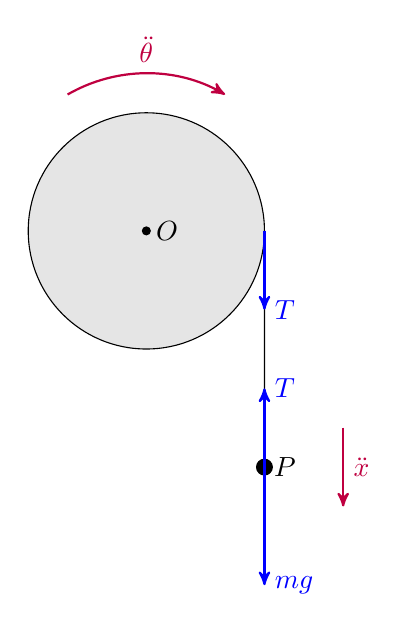
\begin{tikzpicture}[scale=1]
		\draw[fill=gray!20] (0,0)node[right]{$O$} circle (1.5);
		\draw[fill] (0,0) circle(0.05);
		\draw[fill] (1.5,0) -- ++ (0,-3) circle(0.1) node[right]{$P$};
		\draw[thick, ->,purple] (120:2) arc(120:60:2);
		\node[purple] at (0,2.3){$\ddot{\theta}$};
		\draw[thick,purple,->] (2.5,-2.5) --++ (0,-1) node[right,midway]{$\ddot{x}$}; 
		\draw[thick,blue,->] (1.5,-3) --++ (0,-1.5) node[right]{$mg$};
		\draw[thick,blue,->] (1.5,-3) --++ (0,1) node[right]{$T$};
		\draw[thick,blue,->] (1.5,0) --++ (0,-1) node[right]{$T$};
		\end{tikzpicture}
		%Example \ref{ex-rotdisc}
	\end{center}
\end{figure}

for particle: $mg-T=m\ddot{x}$

for disc: $\tau = I \ddot{\theta} \RA T\cdot R = \frac{1}{2}MR^2 \cdot \ddot{\theta} \RA T = \frac{1}{2}MR \cdot \ddot{\theta}$

together with $\ddot{x}=\ddot{\theta} R$, we have: $mg - \frac{1}{2}MR\ddot{\theta} = m\ddot{\theta} R \RA \ddot{\theta} = \frac{2mg}{(2m+M)R}$ \eoe



\subsection{rotational energy}

\subsubsection{rotational kinetic energy}

for a rigid body rotating about some axis, its K.E.: $E_k = \sum_i \frac{1}{2}\Delta m_i v_i^2 = \sum_i \frac{1}{2}\Delta m_i (\omega r_i)^2$

same angular speed $\omega$ throughout, so $E_k = \frac{1}{2} \big(\sum_i r_i^2 \Delta m_i\big) \omega^2$

note that $\sum_i r_i^2 \Delta m_i$ gives the moment of inertia $I$

hence rotational kinetic energy of a rigid body is: $\boxed{E_k = \frac{1}{2} I \omega^2}$

\subsubsection{conservation of mechanical energy}

for rotational motion, conservation of mechanical energy still holds if no energy loss to friction

i.e., change in G.P.E equals change in K.E.

G.P.E. change can be found by comparing initial and final positions of c.o.m.

K.E. change can be computed using new formula $E_k = \frac{1}{2} I \omega^2$

\example{The same rigid-body system as in Example \ref{ex-lollipop} is released from rest from a horizontal position. What is the maximum speed for the particle during the subsequent motion?}

greatest speed when the system becomes downward vertical

increase in K.E. equals loss in G.P.E.: 

{
\centering

$\frac{1}{2}I\omega^2 - 0 = 4mg\cdot \frac{3}{2}a + 5mg\cdot4a+2mg\cdot5a$

$\frac{1}{2}\cdot 144ma^2 \cdot \omega^2 = (6+20+10)mga \RA \omega_\tmax = \sqrt{\frac{g}{2a}}$

}

for the particle: $v_\tmax = \omega_\tmax r = \sqrt{\frac{g}{2a}} \cdot 5a \RA  v_\tmax = \sqrt{\frac{25ga}{2}}$ \eoe

\subsection{small-amplitude oscillations}

when a rigid-body system is displaced from vertical equilibrium by a small angle

it can be shown that the motion is approximately simple harmonic

to do this, the following step-by-step guide is given for reference

\begin{compactenum}
	\item find moment of inertia of the system about the point of suspension
	
	\item when system is displaced by angle $\theta$ from rest position, find resultant torque acting
	
	\item write down equation of motion $\tau = I \ddot{\theta}$, and solve for angular acceleration $\ddot{\theta}$
	
	usually it takes the form $\ddot{\theta} = - \omega^2 \sin\theta$, where $\omega^2$ is some constant with dimension $T^{-2}$
	
	\item apply small-angle approximation ($\sin\theta \approx \theta$ for small $\theta$), one gets $\ddot{\theta} \approx - \omega^2 \theta$
	
	\item identify that this is approximately simple harmonic, period of oscillation can then be found
\end{compactenum}


\example{The same rigid-body system as in Example \ref{ex-lollipop} is slightly displaced from its equilibrium position, show that it performs simple harmonic oscillation provided the angular displacement is small. }

\begin{wrapfigure}{l}{0.3\textwidth}
\begin{center}
	\vspace*{-5pt}
	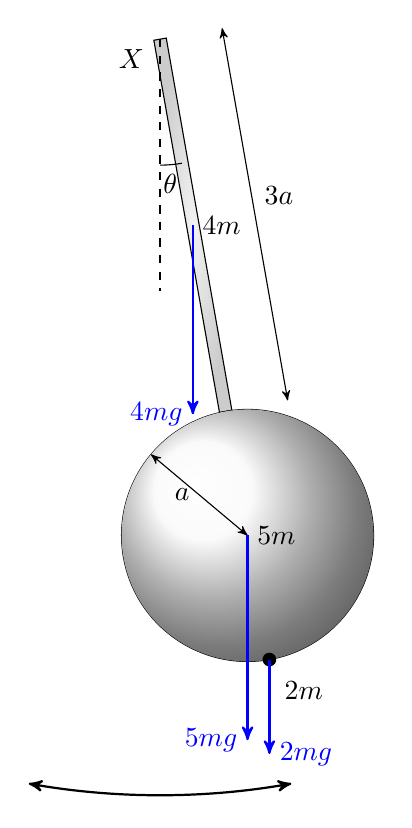
\begin{tikzpicture}[scale=0.8]
	\shadedraw[inner color=gray!10, outer color=gray!40, draw=black,rotate=-80] (0,-0.1) node[below left]{$X$} rectangle (6,0.1);
	\draw[rotate=-80] (8,0) circle (2);
	\shade[ball color = gray!5,rotate=-80] (8,0) circle (2);
	\draw[fill,rotate=-80] (10,0) circle(0.1);
	\draw[<->,rotate=-80] (0,1) --++ (6,0) node[midway,above right]{$3a$};
	\draw[<->,rotate=-80] (8,0) --++ (-140:2) node[midway,left]{$a$};
	\node[right] at (-80:3) {$4m$};
	\node[right] at (-80:8) {$5m$};
	\node[right] at (-80:10.5) {$2m$};
	\draw[thick, <->] (-80:12) arc(-80:-100:12);
	\draw[->,thick,blue] (-80:3) --++ (0,-3) node[left]{$4mg$};
	\draw[->,thick,blue] (-80:8) --++ (0,-3.25) node[left]{$5mg$};
	\draw[->,thick,blue] (-80:10) --++ (0,-1.5) node[right]{$2mg$};
	\draw[dashed] (0,0) -- (0,-4);
	\draw (-80:2) arc(-80:-90:2);
	\node at (-86:2.3) {$\theta$};
\end{tikzpicture}
\end{center}
\vspace*{-15pt}
\end{wrapfigure}

moment of inertia is found to be: $I=144ma^2$

when displaced by $\theta$, magnitude of net torque on system is

{
\centering

$\tau = 4mg\cdot\frac{3}{2}a\sin\theta + 5mg\cdot4a\sin\theta + 2mg\cdot5a\sin\theta$

$\tau = 36 mga\sin\theta$

}

note angular displacement is counter-clockwise, while torque acts in clockwise direction, equation of motion $\tau = I \ddot{\theta}$ reads:

{
	\centering
	
	$-36mga\sin\theta = 144ma^2 \cdot \ddot{\theta} \RA \ddot{\theta} = -\frac{g}{4a}\sin\theta$
	
}

given that $\theta \approx 0$, then $\sin\theta \approx \theta$ (small-angle approximation)

{
	\centering
	
	$\ddot{\theta} \approx -\frac{g}{4a}\theta$
	
}

this performs approximate simple harmonic motion

angular frequency: $\omega = \sqrt{\frac{g}{4a}} = \frac{1}{2}\sqrt{\frac{g}{a}}$

period of oscillation: $T=\frac{2\pi}{\omega} \RA T=4\pi\frac{a}{g}$ \eoe


\example{A uniform annulus lamina is formed by removing a disc of radius $a$ from a disc of radius $2a$ of mass $m$. The lamina is free to rotate about a horizontal axis $l$ tangential to the outer rim and in the plane of the lamina. (a) Find the moment of inertia of this rigid body about axis $l$. (b) Show that small oscillations about axis $l$ are approximately simple harmonic, and find its period. (c) When hanging at rest, with $O$ vertically below $l$, the lamina is given an angular speed $\omega_0$ about $l$. If the lamina completes full circle, what is the minimum value of $\omega_0$?} \label{ex-annulus}

\begin{figure}[htp]
	\begin{center}
		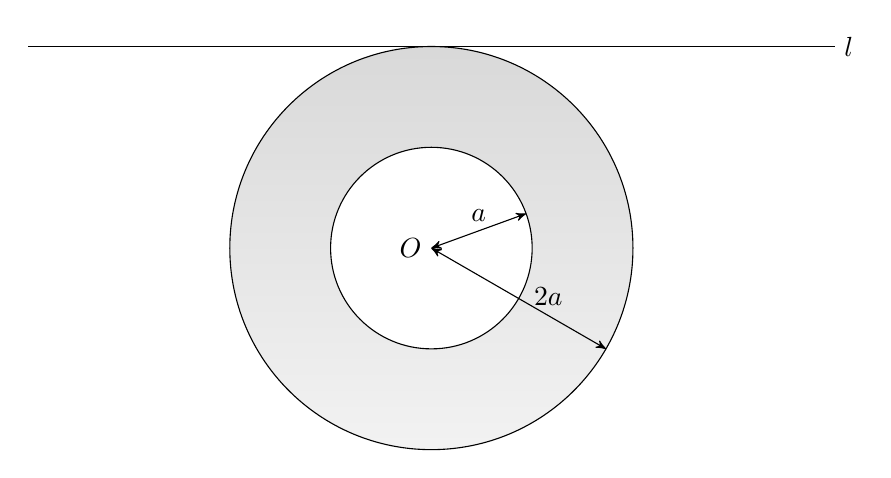
\begin{tikzpicture}[scale=0.64]
		\shadedraw[top color=gray!30,bottom color=gray!10, draw=black] (0,0) circle(4);
		\draw[fill=white] (0,0) node[left]{$O$} circle(2);
		\draw (-8,4) -- (8,4) node[right]{$l$};
		\draw[<->] (0,0) -- (20:2) node[midway,above]{$a$};
		\draw[<->] (0,0) -- (-30:4) node[pos=0.67,above]{$2a$};
		\end{tikzpicture}
		%Example \ref{ex-annulus}
	\end{center}
\end{figure}

\vspace*{-0.5\baselineskip}

apply perpendicular axis and parallel axis theorem for the full disc and the removed part\footnote{Note that the axis through $O$ parallel to $l$ lies within plane of lamina, we need to use perpendicular axis theorem to find the moment of inertia about this axis, then use parallel axis theorem to find the moment of inertia about $l$.}:

{

\centering

$I_\text{disc} = \frac{1}{2}\cdot \frac{1}{2} m(2a)^2 + m(2a)^2 = 5ma^2, \quad I_\text{removed} = \frac{1}{2}\cdot \frac{1}{2}\frac{m}{4}a^2 + \frac{m}{4}(2a)^2 = \frac{17}{16}ma^2$

$I = I_\text{disc} - I_\text{removed} = 5ma^2 - \frac{17}{16}ma^2 \RA I= \frac{63}{16}ma^2$

}

when displaced by $\theta$ from downward vertical, equation of motion $\tau = I \ddot{\theta} $ can be written as:

{

\centering

$ - \frac{3m}{4}g\cdot2a\sin\theta = \frac{63}{16}ma^2 \cdot \ddot{\theta} \RA \ddot{\theta} = -\frac{8g}{21a}\sin\theta$

}

apply small-angle approximation $\sin\theta\approx\theta$, we have: $\ddot{\theta} = -\frac{8g}{21a}\theta$

so the annulus describes approximate simple harmonic motion, and its period is

{
	
\centering

$T=\frac{2\pi}{\omega}=2\pi\sqrt{\frac{21a}{8g}} \RA T=\pi\sqrt{\frac{21a}{2g}}$

}

to complete full turn, the annulus must reach highest position where $O$ is vertically above $l$

consider conservation of energy: $\Delta E_k = \Delta E_p$, we have:

{
	
\centering
	
$ \frac{1}{2}I\omega_0^2 - \frac{1}{2}I\omega^2 = \frac{3}{4}mg\cdot 4a \RA \omega_0^2 = \omega^2 + \frac{6mga}{I} = \omega^2 + \frac{32g}{21a} \RA \omega_0^2 \geq \frac{32g}{21a}$
	
}

minimum value of $\omega_0$ is therefore $\omega_{0,\tmin} = \frac{32g}{21a}$ \eoe

\subsection{analogy with linear motion}

\vspace*{0.5\baselineskip}

\begin{center}
	{\renewcommand{\arraystretch}{1.2}
	\renewcommand{\tabcolsep}{0.2cm}
	\begin{tabular}{|c|c|c|}
	\hline
	 & linear motion & rotational motion \\ \hline
	position & displacement $x$ & angular displacement $\theta$ \\ \hline
	state of motion & velocity $v$ & angular velocity $\omega$ \\ \hline
	change of state & acceleration $a$ & angular acceleration $\alpha$ \\ \hline
	interaction & force $F$ & torque/moment $\tau$ \\ \hline
	inertia & mass $m$ & moment of inertia $I$ \\ \hline \hline
	equation of motion & $F=ma$ & $\tau = I \alpha$ \\ \hline
	kinetic energy & $E_k = \frac{1}{2}mv^2$ & $E_k = \frac{1}{2}m\omega^2$ \\ \hline
	work done & $W=Fx$ & $W=\tau \theta$ \\ \hline
	\end{tabular}}
\end{center}

\section{Equilibrium}

\subsection{mechanical equilibrium}

equilibrium means no translational or rotational acceleration

equilibrium conditions are: $\boxed{\sum F = 0}$ and $\boxed{\sum \tau = 0}$

no resultant force: net force in any direction cancels out

no resultant torque: clockwise and anti-clockwise torques cancel out about any point

for a system of objects, one can take any single object or treat entire system as a whole

when treating individual objects, should consider internal forces between one and another

note internal forces always come in pairs (Newton’s 3$^\text{rd}$ law, action-reaction principle)

when treating whole system, only external forces are important

\subsection{frictional forces}

static friction is a self-adjustive force that always opposes trend of relative motion

maximum static friction depends on roughness of surface and strength of contact force

empirical rule states that $\boxed{f \leq f_\text{lim} = \mu N}$ , where $f_\text{lim}$ is called limiting friction

$\mu$ is called coefficient of friction, rough surfaces have larger values of $\mu$

for equilibrium, i.e., object does not slide over surfaces, one requires $\boxed{\mu \geq \frac{f}{N}}$

\subsubsection*{tips for solving equilibrium problems}

\begin{compactitem}
	\item when you encounter a force of unknown magnitude acting at some bizarre angle (force at a hinge or a rough peg, tension at end of a beam, etc.), taking moments about where this force acts might be a good idea to get around it
	
	\item for a system with several mutually interacting objects, write down equilibrium equations for the system as a whole might lead to a breakthrough
	
	\item sometimes you need to solve a set of simultaneous equations to determine one particular force, when you find any one of your equation does not work out, just stay patient and try a few more
	
	\item last but not least, don't panic, you have all the freedom to try to write down a whole set of equations, some of them will eventually work out
\end{compactitem}

\example{a uniform rod $AC$ of length $8a$ and weight W rests in equilibrium against surface of a smooth cylinder, which is against a vertical wall. The rod is inclined at an angle $\theta$ to a rough horizontal plane, where $\cos\theta=\frac{3}{5}$. A particle of weight $kW$ is attached to the rod at $C$. Given that $AB = 5a$, and the value of coefficient of friction between the rod and the ground is $\mu = \frac{3}{4}$. Find the set of values of $k$ for which equilibrium is possible.} \label{ex-rodball}

\begin{figure}[htp]
	\begin{center}
		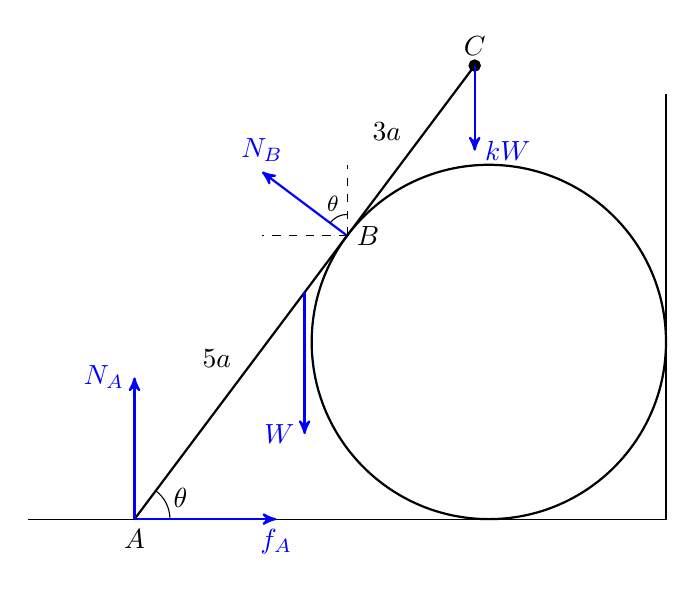
\begin{tikzpicture}[scale=0.9]
		\draw[thick] (0,0) circle (2.5);
		\draw[thick] (-5,-2.5) node[below] {$A$} --++ (4.8,6.4);
		\draw (-6.5,-2.5) --++ (9,0) --++ (0,6);
		\draw[fill] (-0.2,3.9) circle(0.08) node[above] {$C$};
		\draw[thick,blue,->] (-5,-2.5) --++ (0,2) node[left]{$N_A$};
		\draw[thick,blue,->] (-5,-2.5) --++ (2,0) node[below]{$f_A$};
		\draw[thick,blue,->] (-2,1.5) --++ (-1.2,0.9) node[above]{$N_B$};
		\draw[thick,blue,->] (-2.6,0.7) --++ (0,-2) node[left]{$W$};
		\draw[thick,blue,->] (-.2,3.9) --++ (0,-1.2) node[right]{$kW$};
		\draw (-4.5,-2.5) arc(0:53.13:0.5);
		\node at (-4.35,-2.2) {$\theta$};
		\node[right] at (-2,1.5) {$B$};
		\node[above left] at (-3.5,-0.5) {$5a$};
		\node[above left] at (-1.1,2.7) {$3a$};
		\draw[dashed] (-2,1.5) --++ (-1.2,0);
		\draw[dashed] (-2,1.5) --++ (0,1);
		\draw (-2,1.8) arc(90:143.13:0.3);
		\node at (-2.2,1.95) {{\footnotesize $\theta$}};
		\end{tikzpicture}
%		
%		Example \ref{ex-rodball}
	\end{center}
\end{figure}

\vspace*{-1\baselineskip}

take moments about $A$:

{
	
	\centering
	
	$N_B \cdot 5a = W \cdot 4a\cos\theta + kW \cdot 8a \cos\theta$
	
	$5N_B = 4\cdot\frac{3}{5}W + 8\cdot\frac{3}{5}kW \RA N_B = \frac{12+24k}{25}W$
	
}

resolve horizontally:

{
	
	\centering
	
	$f_A = N_B\sin\theta \RA f_A = \frac{12+24k}{25}W \times \frac{4}{5} \RA f_A = \frac{48+96k}{125}W$
	
}

resolve vertically:

{
	
	\centering
	
	$N_A + N_B \cos\theta = W + kW \RA N_A = W+kW -\frac{12+24k}{25}W \cdot \frac{3}{5} \RA N_A = \frac{89+53k}{125}W$
	
}

no sliding between rod and ground requires:

{
	
	\centering
	
	$f_A\leq \mu N_A \RA \frac{48+96k}{125}W \leq \frac{3}{4}\times \frac{89+53k}{125}W \RA 4(48+96k) \leq 3(89+53k)$
	
	$\RA 192 + 384k \leq 267 + 159k \RA 225k \leq 75 \RA k\leq \frac{1}{3}$
	
}

so range for values of $k$ is $0<k\leq \frac{1}{3}$ \eoe

\newpage

\vspace*{-1.2\baselineskip}

\example{Two uniform rods $AB$ and $AC$ are smoothly hinged at $A$. Rod $AB$ has length $8a$ and weight $3W$. Rod $AC$ has length $6a$ and weight $2W$. The rods are in equilibrium in a vertical plane with $B$ and $C$ resting on a rough horizontal plane and angle $CAB$ forms a right angle. (a) Find the force between the two rods at the hinge $A$. (b) The coefficient of friction between each rod and the floor is $\mu$. Find the least possible value of $\mu$.} \label{ex-tworods}

\begin{figure}[htp]
	\begin{center}
		\begin{tikzpicture}[scale=1]
		\draw (-2,0) -- (12,0);
		\draw[thick] (0,0) node[below]{$B$} -- (3.2,2.4) node[midway,above left]{$4a$} -- (6.4,4.8) node[above]{$A$} node[midway, above left]{$4a$} -- (8.2,2.4) node[midway,above right]{$3a$} -- (10,0) node[below]{$C$} node[midway,above right]{$3a$};
		\draw[thick,blue,->] (3.2,2.4) --++ (0,-1.5) node[right]{$3W$};
		\draw[thick,blue,->] (8.2,2.4) --++ (0,-1) node[left]{$2W$};
		\draw[thick,blue,->] (0,0) --++ (1.5,0) node[below]{$f_B$};
		\draw[thick,blue,->] (0,0) --++ (0,1.5) node[left]{$N_B$};
		\draw[thick,blue,->] (10,0) --++ (-1.5,0) node[below]{$f_C$};
		\draw[thick,blue,->] (10,0) --++ (0,1.5) node[right]{$N_C$};
		\draw[thick,blue,->] (6.3,4.8) --++ (-0.8,1.6) node[left]{$F_A$};
		\draw[thick,blue,->] (6.4,4.7) --++ (0.8,-1.6) node[left]{$F_A$};
		\end{tikzpicture}
%		
%		Example \ref{ex-tworods}
	\end{center}
\end{figure}

\vspace*{-1\baselineskip}

take moments about $C$ for system:

{

\centering

$3W\cdot\left(4a\cos\theta+6a\sin\theta\right)+2W\cdot(3a\sin\theta)=N_B\cdot 10a$

$3W\cdot(4a\times\frac{4}{5}+6a\times\frac{3}{5})+2W\cdot(3a\times\frac{3}{5}) = N_B \cdot 10a$

$10 N_B = \left(\frac{48}{5} + \frac{54}{5} + \frac{18}{5}  \right) = 24 W \RA N_B = \frac{12}{5}W$

} 

take moments about $A$ for rod $AB$:

{
	
\centering
	
$N_B\cdot 8a\cos\theta = 3W\cdot 4a\cos\theta + f_B \cdot 8a\sin\theta$

$\frac{12}{5}W \cdot 8a\cdot\frac{4}{5} = 3W \cdot 4a\cdot\frac{4}{5} + f_B \cdot 8a\cdot\frac{3}{5}$

$\frac{96}{5}W = 12W + 6f_B \RA f_B = \frac{6}{5}W$
	
}

resolve horizontally for rod $AB$:

{
	
\centering
	
$F_{A,x} = f_B \RA F_{A,x} = \frac{6}{5}W$
	
}

resolve vertically for rod $AB$:

{
	
\centering
	
$N_B + F_{A,y} = 3W \RA F_{A,y} = 3W - \frac{12}{5}W = \frac{13}{5}W$
	
}

hence we find interaction at hinge $A$:

{
	
\centering
	
$F_A = \sqrt{F_{A,x}^2 + F_{A,y}^2} = \sqrt{\left(\frac{6}{5}W\right)^2 + \left(\frac{13}{5}W\right)^2} \RA F_A = \frac{\sqrt{205}}{5}W$
	
}

resolve horizontally for system:

{
	
\centering
	
$f_C = f_B \RA f_C = \frac{6}{5}W$
	
}

resolve vertically for system:

{
	
\centering
	
$N_B + N_C = 3W + 2W \RA N_C = 5W - \frac{12}{5}W \RA N_C = \frac{13}{5}W$
	
}

at contact $B$ and $C$, using $\mu \geq \frac{f}{N}$

{
	
\centering

$\mu_B \geq \frac{\frac{6}{5}W}{\frac{12}{5}W}=\frac{1}{2} \quad$ and $\quad$ $\mu_B \geq \frac{\frac{6}{5}W}{\frac{13}{5}W}=\frac{6}{13}$

}

no sliding at either $B$ or $C$ requires $\mu \geq \tmax(\mu_B, \mu_C)$, so $\mu \geq \frac{6}{13}$ \eoe

%\newpage
%
%\vspace*{-\baselineskip}

\example{A uniform rod $AB$ of weight $W$ and length $2a$ rests on a rough horizontal plane. A light inextensible string $BC$ is attached to the rod at $B$ and passes over a small smooth fixed peg $P$, which is at a distance $3a$ vertically above end $A$. A particle of weight $kW$ is attached at $C$ and hangs vertically. $A$, $B$ and $C$ are in the same vertical plane. In equilibrium the rod is inclined at an angle $\theta$ to the
horizontal where $\sin\theta=\frac{3}{5}$. (a) Given that the system is in limiting equilibrium, find the coefficient of friction between the rod and the plane is $\mu$. (B) Find the value of $k$.}

\begin{figure}[htp]
	\begin{center}
		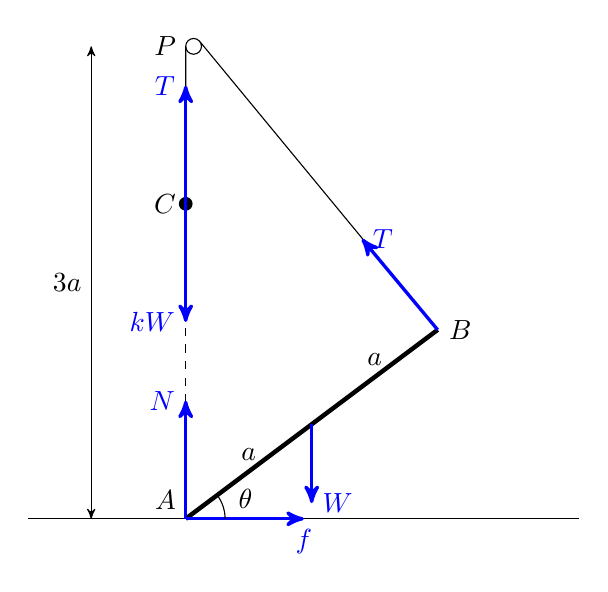
\begin{tikzpicture}[scale=1]
		\draw (-2,0) -- (5,0);
		\draw[dashed] (0,0) node[above left]{$A$} -- (0,6) node[left]{$P$};
		\draw[fill] (0,4) circle(0.08) node[left]{$C$} -- (0,6);
		\draw[ultra thick] (0,0) -- (1.6,1.2) node[midway,above]{$a$} -- (3.2,2.4) node[right]{$B$} node[midway,above]{$a$};
		\draw (0.1,6) circle(0.1) ++ (42:0.1) -- (3.2,2.4);
		\draw[very thick,blue,->] (0,0) --++ (1.5,0) node[below]{$f$};
		\draw[very thick,blue,->] (0,0) --++ (0,1.5) node[left]{$N$};
		\draw[very thick,blue,->] (1.6,1.2) --++ (0,-1) node[right]{$W$};
		\draw[very thick,blue,->] (3.2,2.4) --++ (129.8:1.5) node[right]{$T$};
		\draw[very thick,blue,->] (0,4) --++ (0,-1.5) node[left]{$kW$};
		\draw[very thick,blue,->] (0,4) --++ (0,1.5) node[left]{$T$};
		\draw (0.5,0) arc(0:36.87:0.5);
		\node at (18:0.8) {$\theta$};
		\draw[<->] (-1.2,0) --++ (0,6) node[left,midway]{$3a$};
		\end{tikzpicture}
	\end{center}
\end{figure}

\vspace*{-1\baselineskip}

take moments about $P$ for the rod:

{

\centering

$f\cdot3a = W\cdot a\cos\theta \RA f=\frac{1}{3}W\cos\theta = \frac{1}{3}W\cdot\frac{4}{5} \RA f=\frac{4}{15}W$

}

take moments about $B$ for the rod:

{

\centering

$N\cdot2a\cos\theta = f\cdot2a\sin\theta + W\cdot a\cos\theta$

$2N\cdot\frac{4}{5} = 2\cdot\frac{4}{15}W\cdot\frac{3}{5} + W\cdot\frac{4}{5} \RA N=\frac{7}{10}W$

}

limiting friction so $\mu = \frac{f}{N} = \frac{4}{15} \cdot \frac{10}{7} \RA \mu = \frac{8}{21}$

resolve horizontally for rod: $T_x = f \RA T_x = \frac{4}{15}W$

resolve vertically for rod: $T_y + N = W \RA T_y = W - \frac{7}{10}W \RA T_y = \frac{3}{10}W$

tension in string is: $T = \sqrt{T_x^2+T_y^2} = \sqrt{\left(\frac{4}{15}\right)^2 + \left(\frac{3}{10}\right)^2} \cdot W \RA T=\frac{\sqrt{145}}{30}W$

equilibrium for particle $C$ requires $T=kW$, so $k=\frac{\sqrt{145}}{30}$ \eoe

\section{Mega Examples}

in some cases, one needs combined knowledge from several sections to solve a problem

in this section, we walk through a few long questions to consolidate thinking

\example{A particle $P$ of mass $m$ rests on a smooth horizontal table, and is connected to a fixed point $A$ by an elastic string of natural length $2a$ and modulus of elasticity $mg$. When the particle is at its rest position $O$, it is given an impulse of magnitude $m\sqrt{\frac{ga}{2}}$ and $P$ starts to move away from $A$ towards a barrier $B$. The barrier is at a distance of $\frac{1}{2}a$ from $O$. The coefficient of restitution between the particle and the barrier is $\frac{1}{\sqrt{3}}$. Find the time when $P$ first returns to $O$.}

\begin{figure}[htp]
	\begin{center}
		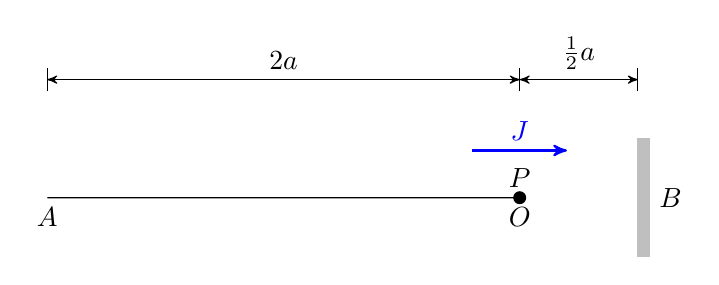
\begin{tikzpicture}[scale=1.5]
		\draw[fill] (0,0)node[below]{$A$} -- (4,0) circle(0.05) node[above]{$P$} node[below]{$O$};
		\draw[gray!50,fill] (5,-0.5) rectangle (5.1,0.5);
		\node[right] at (5.1,0) {$B$};
		\draw[<->] (0,1) -- (4,1) node[midway, above]{$2a$};
		\draw[<->] (4,1) -- (5,1) node[midway, above]{$\frac{1}{2}a$};
		\draw (0,0.9) --++ (0,0.2);
		\draw (4,0.9) --++ (0,0.2);
		\draw (5,0.9) --++ (0,0.2);
		\draw[blue,thick,->] (3.6,0.4) --++ (0.8,0) node[midway, above]{$J$};
		\end{tikzpicture}
	\end{center}
\end{figure}

motion of $P$ consists of three stages: motion from $O$ to $B$ (part of simple harmonics), impact with barrier, and motion from $B$ to $O$ (also simple harmonic, but with a different amplitude)

we first write down the equation of motion when $OP = x$, :

{

\centering

$m\ddot{x} = -\frac{\lambda}{l_0}x \RA m\ddot{x} = -\frac{mg}{2a}x \RA \ddot{x} = -\frac{g}{2a}x$

}

so $P$ describes simple harmonic motion along $OB$ with angular frequency $\omega = \sqrt{\frac{g}{2a}}$

at $t=0$, impulse-momentum relation reads: $J=m\sqrt{\frac{ga}{2}}=mu_0 \RA u_0 = \sqrt{\frac{ga}{2}}$

from $O$ to $B$, amplitude of motion is: $x_0 = \frac{u_0}{\omega} = \sqrt{\frac{ga}{2}} \cdot \sqrt{\frac{2a}{g}} \RA x_0 = a$

displacement-time relation is: $x(t)=x_0\sin\omega t \RA x(t)=a\sin\omega t $

just before hitting barrier, $x=\frac{1}{2}a$, so

{

\centering

$a\sin\omega t_1 = \frac{1}{2}a \RA \omega t_1 = \sin^{-1}\tfrac{1}{2} \RA t_1 = \frac{\pi}{6\omega}$

$u = \omega\sqrt{x_0^2-x^2} = \sqrt{\frac{g}{2a}} \cdot \sqrt{a^2-\frac{1}{4}a^2} \RA u=\sqrt{\frac{3ga}{8}}$

}

after hitting barrier: $v = -eu = -\frac{1}{\sqrt{3}}\cdot \sqrt{\frac{3ga}{8}} \RA v = -\sqrt{\frac{ga}{8}}$

{
	
\centering
	
$v^2 = \omega\sqrt{x_0^2-x^2} \RA x'_0 = \sqrt{\frac{v^2}{\omega^2} + x^2} = \sqrt{\frac{ga}{8} \cdot\ \frac{2a}{g} + \frac{1}{4}a^2} \RA x'_0 = \frac{1}{\sqrt{2}}a$

}

so as $P$ travels from $B$ back to $O$, amplitude becomes smaller

note that it takes the same time for $P$ to move from $O$ to $B$ as long as amplitude is fixed

we can use displacement-time relation $x'(t)=x'_0\sin\omega t$, or  $x'(t)=\frac{1}{\sqrt{2}}a\sin\omega t$, to find:

{
	
\centering
	
$ \frac{1}{\sqrt{2}}a\sin\omega t_2 = \frac{1}{2}a \RA \omega t_2 = \sin^{-1}\tfrac{1}{\sqrt{2}} \RA t_2 = \frac{\pi}{4\omega}$
	
}

total time taken: $t=t_1+t_2 = \frac{\pi}{6\omega}+\frac{\pi}{4\omega} = \frac{5\pi}{12\omega} \RA t=\frac{5\pi}{12} \sqrt{\frac{2a}{g}}$ \eoe
	
\example{A uniform disc of radius $a$ and mass $2m$ is free to rotate in a vertical plane about a horizontal axis through its centre $O$. A particle $P$ of mass $m$ is placed on the highest point of the rough edge of the disc. The system is slightly disturbed so that $OP$ begins to rotate. For the subsequent motion, the particle remains in contact with the disc without slipping. (a) When OP makes an angle $\theta$ with the upward vertical, find $\dot{\theta}$ and $\ddot{\theta}$ in terms of $g$ and $\theta$. (b) Given that the coefficient of friction between the particle and the disc is $\mu=\frac{1}{4}$, find the angle $\theta$ when $P$ just begins to slip. (c) Show that, however large the value of $\mu$, the particle cannot lose contact with the disc before it starts to slip.}

\begin{figure}[htp]
	\begin{center}
		\begin{tikzpicture}[scale=0.8]
		\draw (0,0) node[below]{$O$} circle(4);
		\draw[dashed] (0,4) -- (0,0) node[midway,left]{$a$} -- (60:4) node[midway,right]{$a$};
		\draw[fill] (60:4.1) circle(0.1) node[right]{$P$};
		\node at (75:1.1) {$\theta$};
		\draw (0,0.8) arc(90:60:0.8);
		\draw[blue,thick,->] (60:4.1) --++ (0,-2.5) node[right]{$mg$};
		\draw[blue,thick,->] (60:4.1) --++ (60:1.5) node[right]{$N$};
		\draw[blue,thick,->] (60:4.1) --++ (150:1) node[above]{$f$};
		\end{tikzpicture}
	\end{center}
\end{figure}

\vspace*{-0.5\baselineskip}

moment of inertia of system is:

{
	
	\centering
	
	$I = I_\text{disc} + I_P = \frac{1}{2}\cdot2ma^2 + ma^2 \RA I = 2ma^2$
	
	
}

to find $\dot{\theta}$, consider energy changes, loss in G.P.E. for particle becomes rotational K.E. of system:

{

\centering

$mga(1-\cos\theta) = \frac{1}{2}I\dot{\theta}^2 \RA mga(1-\cos\theta) = \frac{1}{2} \cdot 2ma^2 \cdot \dot{\theta}^2 \RA \dot{\theta}^2 = \frac{g(1-\cos\theta)}{a} $

}

to find $\ddot{\theta}$, consider torque acting on system:

{

\centering

$\tau = I\ddot{\theta} \RA mga\sin\theta = 2ma^2\cdot\ddot{\theta} \RA \ddot{\theta} = \frac{g\sin\theta}{2a}$

}

or one can take time derivative for $\dot{\theta}^2$ to find:

{

\centering

$\ddt{\dot{\theta}^2} = \opdt\left(\frac{g(1-\cos\theta)}{a}\right)  \RA 2\dot{\theta}\cdot\ddot{\theta} = \frac{g\sin\theta\cdot\dot{\theta}}{a} \RA \ddot{\theta} = \frac{g\sin\theta}{2a}$

}

to find friction and contact force on $P$, consider tangential and centripetal forces on $P$:

{

\centering

$mg\sin\theta - f = m\cdot a\ddot{\theta} \RA f = mg\sin\theta - m\cdot \frac{1}{2}g\sin\theta \RA f= \frac{1}{2}mg\sin\theta$

$mg\cos\theta - N = m\dot{\theta}^2 a \RA N = mg\cos\theta - mg(1-\cos\theta) \RA N = mg(2\cos\theta -1) $ ($\Delta$)

}

when $P$ is about to slip, frictional force is at limiting value $f=\mu N$

{

\centering

$\frac{1}{2}mg\sin\theta = \mu mg(2\cos\theta -1) \RA \sin\theta = 4\mu\cos\theta -2\mu \RA 4\mu\cos\theta -\sin\theta = 2\mu$ (\#)

}

to find limiting $\theta$, substitute $\mu=\frac{1}{4}$, we find

{

\centering

$\cos\theta - \sin\theta = \frac{1}{2} \RA \sqrt{2}\cos(\theta+45^\circ)=\frac{1}{2} \RA \theta = \cos^{-1}\tfrac{1}{2\sqrt{2}} - 45^\circ \RA \theta \approx 24.3^\circ$

}

rewrite (\#) as $\cos\theta = \frac{2\mu+\sin\theta}{4\mu}$, and plug this into ($\Delta$):

{

\centering

$N = mg\left(2\cdot \frac{2\mu+\sin\theta}{4\mu} - 1\right) = mg\left(1 + \frac{\sin\theta}{2\mu} -1 \right) \RA N = \frac{mg\sin\theta}{2\mu}$

}

obviously $N>0$, so $P$ will not lose contact before slipping occurs \eoe

%\newpage
%\printindex

\end{document}
